\exercisesection{}

\begin{enumerate}
\def\labelenumi{\arabic{enumi})}
\item
  设 G 为一个局部紧群，H 为 G 的闭子群。对 \(\xi\in H\)，置 \(\chi(\xi)=\Delta_{H}(\xi)\Delta_{G}(\xi)^{-1}\)。把 H 看作通过平移在 G 上右作用。证明在 \(\mathcal{K}^{\chi}(G)\) 上存在一个非零正线性型 I；除相差一个常数因子外，这样的线性型只有一个，而且它在左平移下不变。（使用命题 3，其中 X=G，并取 \(\mu\) 为 G 的左 Haar 测度。）
\item
  设 X 和 \(X'\) 是两个局部紧空间，局部紧群 H 在其中连续且适当地右作用。令 \(\theta\) 为从 X 到 \(X'\) 的适当连续映射，它与 H 的恒等映射相容（GT, III, §2, No.~4），并令 \(\theta': X/H \to X'/H\) 为由 \(\theta\) 通过取商得到的映射。设 \(f'\) 是 \(X'\) 上的连续函数，其支集与每个紧集的饱和集的交都是紧的。则 \(f = f' \circ \theta\) 在 X 中具有相同性质，并且
\end{enumerate}

\[
f ^ {b} = f ^ {\prime b} = \theta^ {\prime}
\]

（映射 \(f \mapsto f^b\)、\(f' \mapsto f'^b\) 均相对于在 H 上选定的同一个 Haar 测度。）

\begin{enumerate}
\def\labelenumi{\arabic{enumi})}
\setcounter{enumi}{2}
\tightlist
\item
  设 B 为局部紧空间，H 为局部紧群。置 \(\mathbf{X} = \mathbf{B} \times \mathbf{H}\)，群 H 通过下式在 X 上作用：
\end{enumerate}

\[
(b, \xi) \xi^ {\prime} = (b, \xi \xi^ {\prime}).
\]

令 \(\lambda\) 为 \(B = X / H\) 上的测度，\(\beta\) 为 \(H\) 上的左 Haar 测度。则 \(\lambda^{\sharp} = \lambda \otimes \beta\)。

\begin{enumerate}
\def\labelenumi{\arabic{enumi})}
\setcounter{enumi}{3}
\item
  设 X 是局部紧空间，局部紧群 H 在其中连续且适当地右作用。设 \(\beta\) 是 H 上的左 Haar 测度，\(\mu\) 是 X 上满足 \(\geqslant0\) 的测度。设 h 是 X 上满足 \(\geqslant0\) 的连续函数，且 \(h^{b}=1\)。若 f 是 X 上 \(\mu\)-可忽略的满足 \(\geqslant0\) 的函数，则函数 \((x,\xi)\mapsto f(x)h(x\xi)\) 在 X×H 上是 \((\mu\otimes\beta)\)-可忽略的。（存在递减的开集 \(\Omega_{1},\Omega_{2},\ldots\)，使得 \(\mu(\Omega_{n})\) 趋于 0，且 f 在 \(\Omega_{1}\cap\Omega_{2}\cap\cdots\) 之外为零。证明 \(\int^{*}\varphi_{\Omega_{n}}(x)h(x\xi)d\mu(x)d\beta(\xi)\leqslant\mu(\Omega_{n})\)，注意到函数 \((x,\xi)\mapsto\varphi_{\Omega_{n}}(x)h(x\xi)\) 是下半连续的。））
\item
  设 \(\mathbf{G}\) 为局部紧群。对每个 \(s \in \mathbf{G}\)，令 \(\psi_s\) 为加法群 \(\mathbf{R}\) 的自同构，由 \(\psi_s(x) = \Delta_{\mathbf{G}}(s)x\) 定义。令 \(\Gamma\) 为 \(\mathbf{G}\) 与 \(\mathbf{R}\) 的拓扑半直积，由 \(s \mapsto \psi_s\) 定义（GT, III, §2, No.~10）。证明 \(\Gamma\) 是幺模的。
\item
  设 \(G\) 为局部紧群，\(G_1, G_2, G_3\) 为闭子群，且 \(G_3 \subset G_1 \cap G_2\)。假设 \(G, G_1, G_2, G_3\) 都是幺模的，且 \(G_1 / G_3\) 具有有限总测度（对于每个在 \(G_1\) 下不变的测度）。令 \(\lambda, \mu, \nu\) 分别为 \(G / G_1, G / G_2, G_2 / G_3\) 上的不变测度，\(\varphi\) 为 \(G\) 到 \(G / G_1\) 的典范映射。设 \(f \in \mathcal{K}(G / G_1)\)。证明
\end{enumerate}

\[
a \int_ {\mathrm{G} / \mathrm{G} _ {1}} f (u) d \lambda (u) = \int_ {\mathrm{G} / \mathrm{G} _ {2}} d \mu (\dot {x}) \int_ {\mathrm{G} _ {2} / \mathrm{G} _ {3}} f (\varphi (x \xi)) d \nu (\dot {\xi})
\]

\((\dot{x} = x\mathrm{G}_{2}, \dot{\xi} = \xi \mathrm{G}_{3})\)，其中 \(a\) 是与 \(f\) 无关的常数。

¶ 7) a) 设 E 为局部紧空间，Γ 为在 E 上连续左作用的局部紧群。假设对每个 \(x \in E\)，从 Γ 到 E 的映射 \(s \mapsto s \cdot x\) 是适当的，并且 E 上存在一个在 Γ 下不变的非零有界正测度 μ。证明 Γ 是紧的。（设 \((s_n)\) 是 Γ 中点的一个序列。取 E 的一个不被 μ 忽略的紧子集 K。利用 Ch. IV, §4, Exer. 15，证明存在 \(x_0 \in E\)，使得对 n 的无穷多个值有 \(s_n x_0 \in K\)。~由此推出 \((s_n)\) 在 Γ 中有聚点。然后应用 GT, II, §4, Exer. 6。）

\begin{enumerate}
\def\labelenumi{\alph{enumi})}
\setcounter{enumi}{1}
\tightlist
\item
  设 G 为局部紧群，H 和 K 为 G 的两个闭子群。假设 G 和 H 是幺模的，且 G/H 对于 G 下的不变测度具有有限测度。证明 H 和 K 满足 GT, III, §4, Exer. 11 c) 的等价条件，当且仅当 K 是紧的。
\end{enumerate}

\begin{enumerate}
\def\labelenumi{\arabic{enumi})}
\setcounter{enumi}{7}
\tightlist
\item
  设 \(\mathfrak{G}\) 为局部紧群，G 和 H 为 \(\mathfrak{G}\) 的两个闭子群。假设每个 \(s \in \mathfrak{G}\) 都能且只能以一种方式写成 \(s = \xi x = y\eta\) \((\xi, \eta \in \mathbf{G}, x, y \in \mathbf{H})\)，并且 \(\xi, x, y, \eta\) 连续地依赖于 \(s\)。每个 \(\xi \in \mathbf{G}\) 定义 H 到 H 的同胚 \(\widehat{\xi}\)，其定义为 \(\xi x \in \widehat{\xi}(x)\mathbf{G} (x \in \mathbf{H})\)。每个 \(x \in \mathbf{H}\) 定义 G 到 G 的同胚 \(\widehat{x}\)，其定义为 \(\xi x \in \mathrm{H}\widehat{x}(\xi) (\xi \in \mathbf{G})\)。令 \(\mu, \alpha, \beta\) 分别为 \(\mathfrak{G}, \mathbf{G}, \mathbf{H}\) 上的左 Haar 测度。证明
\end{enumerate}

\[
\begin{array}{c} d \widehat {x} ^ {- 1} (\alpha) (\xi) = \frac {\Delta_ {\mathfrak {G}} (\widehat {\xi} (x)) \Delta_ {\mathrm{G}} (\widehat {x} (\xi))}{\Delta_ {\mathrm{H}} (\widehat {\xi} (x)) \Delta_ {\mathrm{G}} (\xi)} d \alpha (\xi), \\ d \widehat {\xi} ^ {- 1} (\beta) (x) = \frac {\Delta_ {\mathrm{G}} (\widehat {x} (\xi))}{\Delta_ {\mathfrak {G}} (\widehat {x} (\xi))} d \beta (x). \end{array}
\]

（取 \(f \in \mathcal{K}(G)\)。说明如下事实：借助 (23) 计算的 \(\int f(u) d\mu(u)\)，无论取 \(X = G\)、\(Y = H\)，还是取 \(X = H\)、\(Y = G\)，当 \(f\) 受到 \(G\) 中元素或 \(H\) 中元素的左平移时都保持不变。）

\begin{enumerate}
\def\labelenumi{\arabic{enumi})}
\setcounter{enumi}{8}
\tightlist
\item
  设 X 为局部紧空间，H 为在 X 上连续（因而适当地）右作用的紧群。记 \(\beta\) 为 H 上的归一化 Haar 测度，记 \(\pi: X \to X/H\) 为典范映射。令 \(\lambda\) 为 X/H 上的正测度，\(\lambda^{\sharp}\) 为 X 上对应的测度。
\end{enumerate}

\begin{enumerate}
\def\labelenumi{\alph{enumi})}
\item
  证明若 N 是 X/H 的 \(\lambda\)-可忽略子集，则 \(\overline{\pi}^{1}(N)\) 是 \(\lambda^{\sharp}\)-可忽略的。（计算集合 \(\overline{\pi}^{1}(U)\) 的测度，其中 U 是 X/H 中的开集。）
\item
  设 \(p\) 是一个有限数且 \(\geqslant 1\)，设 \(f\) 是 \(\mathcal{L}_{\mathrm{F}}^{p}(\mathrm{X},\lambda^{\sharp})\) 中的函数（F 为 Banach 空间，或 \(\mathrm{F} = \overline{\mathbf{R}}\)）。证明那些满足 \(x \in \mathrm{X}\) 且映射 \(\xi \mapsto f(x\xi)\) 关于 \(\beta\) 在 \(\mathrm{H}\) 上不可积的 x 所成的集合具有 \(\overline{\pi}^{1}(\mathrm{N})\) 的形式，其中 \(\mathrm{N}\) 是 \(\lambda\)-可忽略的。此外，若 \(f^b\) 是 \(\mathrm{X / H}\) 上的函数，在几乎处处（相对于 \(\lambda\)）定义，并满足 \(f^b (\pi (x)) = \int_{\mathrm{H}} f(x\xi) d\beta (\xi)\)，则 \(f^b\) 属于 \(\mathcal{L}_{\mathrm{F}}^{p}(\mathrm{X / H},\lambda)\)，且 \(\mathrm{N}_p(f^b)\leqslant \mathrm{N}_p(f)\)。
\item
  反之，若 \(g \in \mathcal{L}_{\mathrm{F}}^{p}(\mathrm{X / H}, \lambda)\)，则函数 \(g \circ \pi\) 属于 \(\mathcal{L}_{\mathrm{F}}^{p}(\mathrm{X}, \lambda^{\sharp})\)。若 \(p, q\) 是共轭指数，\(\mathrm{F}'\) 是 \(\mathrm{F}\) 的对偶，\(f \in \mathcal{L}_{\mathrm{F}}^{p}(\mathrm{X}, \lambda^{\sharp})\) 且 \(g \in \mathcal{L}_{\mathrm{F}'}^{q}(\mathrm{X / H}, \lambda)\)，则
\end{enumerate}

\[
\int_ {\mathrm{X}} \left\langle f (x), g (\pi (x)) \right\rangle d \lambda^ {\sharp} (x) = \int_ {\mathrm{X/H}} \left\langle f ^ {\flat} (z), g (z) \right\rangle d \lambda (z).
\]

\begin{enumerate}
\def\labelenumi{\arabic{enumi})}
\setcounter{enumi}{9}
\tightlist
\item
  采用 §1, No.~6, 命题 6 的记号；对每个 \(\alpha \in A\)，令 \(\mu_{\alpha}\) 为 \(G_{\alpha}\) 上的左 Haar 测度，从而 \(\mu_{\alpha}\) 的逆极限是左 Haar 测度 \(\mu\)，定义在 \(G\) 上。对每个 \(\alpha \in A\)，记 \(\lambda_{\alpha}\) 为 \(K_{\alpha}\) 上的归一化 Haar 测度。
\end{enumerate}

\begin{enumerate}
\def\labelenumi{\alph{enumi})}
\tightlist
\item
  设 \(p\) 是一个有限数且 \(\geqslant 1\)，设 \(f\) 是 \(\mathcal{L}_{\mathrm{F}}^{p}(\mathrm{G},\mu)\) 中的函数（F 为 Banach 空间，或 \(\mathrm{F} = \overline{\mathbf{R}}\)）。对每个 \(\alpha \in \mathbf{A}\)，函数
\end{enumerate}

\[
f _ {\alpha} (s) = \int_ {K _ {\alpha}} f (s \xi) d \lambda_ {\alpha} (\xi),
\]

在几乎处处（相对于 \(\mu\)）定义，属于 \(\mathcal{L}_{\mathrm{F}}^{p}(\mathrm{G},\mu)\)（练习 9）。证明相对于有向集 A，\(f_{\alpha}\) 在 \(p\) 阶均值意义下趋于 \(f\)（使用 §1, No.~6 的引理 2）。

\begin{enumerate}
\def\labelenumi{\alph{enumi})}
\setcounter{enumi}{1}
\tightlist
\item
  假设 A = N 且 p = 1。证明此时 \(f_{n}\) 在 G 中几乎处处（相对于 \(\mu\)）趋于 f（使用类似 Ch. V, §8, Exer. 16 中的方法）。
\end{enumerate}

¶ 11) 设 G 为局部紧群，H 为 G 的闭子群，λ 为 G 上的左 Haar 测度；假设 G/H 上存在一个在 G 下不变的测度 μ，使得 λ = μ \(^{\sharp}\) 且 μ(G/H) \textless{} +∞。令 ν 为 G/H 上满足 \(\nu (\mathrm{G / H}) < +\infty\) 的非零正测度。最后，令 \(h\) 为 \(\mathbf{G}\) 上具有 No.~4, 命题 8 所述性质的函数。

\begin{enumerate}
\def\labelenumi{\alph{enumi})}
\tightlist
\item
  设 A 为 G/H 的 Borel 子集。证明
\end{enumerate}

\[
\int_ {\mathrm{G}} h (s) \nu (s ^ {- 1} \mathrm{A}) d \lambda (s) = \nu (\mathrm{G/H}) \mu (\mathrm{A})
\]

（使用 No.~4 的命题 9 a)。）

\begin{enumerate}
\def\labelenumi{\alph{enumi})}
\setcounter{enumi}{1}
\tightlist
\item
  设 \(A_i\)（\(1 \leqslant i \leqslant n\)）为 \(G / H\) 的 Borel 子集，并对每个 \(i\) 令 \(b_i = \sup_{s \in G} \nu(s^{-1} A_i)\)。证明存在两个不同的指标 \(i, j\)，使得
\end{enumerate}

\[
\int_ {\mathrm{G}} h (s) \nu (s ^ {- 1} \mathrm{A} _ {i}) \nu (s ^ {- 1} \mathrm{A} _ {j}) d \lambda (s) \geqslant \frac {\left(\nu (\mathrm{G} / \mathrm{H})\right) ^ {2}}{\mu (\mathrm{G} / \mathrm{H})} \left(\left(\sum_ {k = 1} ^ {n} \mu (\mathrm{A} _ {k})\right) ^ {2} - \frac {\mu (\mathrm{G} / \mathrm{H})}{\nu (\mathrm{G} / \mathrm{H})} \sum_ {k = 1} ^ {n} b _ {k} \mu (\mathrm{A} _ {k})\right)
\]

（仿照 §1, Exer. 28 a) 论证。）

¶ 12) a) 设 X 为拓扑空间，\(f: X \to N\) 为上半连续函数。令 \(X_0\) 为 X 中 \(f\) 局部常值的点所成的集合，并令 \(Y_0 = X - X_0\)。按如下方式递归地定义 X 的两个子集序列 \((X_i)_{i \geqslant 0}\)、\((Y_i)_{i \geqslant 0}\)：\(X_i\) 是 \(Y_{i-1}\) 中使得 \(f|_{Y_{i-1}}\) 局部常值的点所成的集合，而 \(Y_i = Y_{i-1} - X_i\)。证明 \(X_i\) 是 \(Y_{i-1}\) 的稠密开子集，并且 \(\bigcap_i Y_i = \varnothing\)。

（证明 \(f(x) > i\) 对 \(Y_i\) 的每一点成立。）

\begin{enumerate}
\def\labelenumi{\alph{enumi})}
\setcounter{enumi}{1}
\tightlist
\item
  设 X 为集合，H 为在 X 上右作用的群，\(\pi\) 为 X 到 X/H 的典范映射，并令 A（分别地，B）为所有满足 \(\pi|A:A\to X/H\) 为单射（分别地，为满射）的 A ⊂ X 所成的集合。令 \((V_{1},V_{2},\ldots)\) 为由 A 中元素构成的 X 的可数覆盖。令
\end{enumerate}

\[
\mathrm{V} _ {i} ^ {\prime} = \mathrm{V} _ {i} \cap \complement \left(\mathrm{V} _ {1} \mathrm{H} \cup \mathrm{V} _ {2} \mathrm{H} \cup \dots \cup \mathrm{V} _ {i - 1} \mathrm{H}\right).
\]

证明 \(\mathrm{F} = \bigcup_{i\geqslant 0}\mathrm{V}_i^\prime \in \mathfrak{A}\cap \mathfrak{B}\)。

\begin{enumerate}
\def\labelenumi{\alph{enumi})}
\setcounter{enumi}{2}
\item
  设 X 为局部紧空间，H 为在 X 上连续且适当右作用的可数离散群，\(\pi\) 为 X 到 X/H 的典范映射，\(\mu\) 为 X 上满足 \(\geqslant 0\) 的测度。证明若 b) 中的集合 \(V_{i}\) 是可求积的（Ch. IV, §5, Exer. 17 d)），则 b) 中的集合 F 是一个可求积基本域。
\item
  维持 \(c\) ) 的假设，并使用 No.~10 的记号 \(\mathbf{H}_x, n(x)\)。若对某个 \(x \in X\) 存在 \(V\)，它是 \(x\) 在 \(X\) 中的邻域，使得 \(\mathrm{H}_y = \mathrm{H}_x\) 对所有 \(y \in V\) 成立，则称 x 为一般点。证明 \(X\) 的一般点正是函数 \(n\) 局部常值的点。证明一般点具有一个属于 \(\mathfrak{A}\) 且可求积的开邻域（使用 Ch. IV, §5, Exer. 17 d)）。
\item
  维持 \(c\) ) 的假设，并进一步假设 \(X\) 在无穷远处可数。证明若 \(X - X_0\) 是 \(\mu\)-可忽略的，则存在一个 Borel 且可求积的基本域 \(F\)。（将 \(a\) ) 的构造应用于函数 \(n\)。然后应用 \(c\) ) 和 \(d\) ) 的结果于 \(X_0\)。在每个 \(X_i\) 中作类似论证。）
\item
  设 \(U \in B\) 为开集。证明可以使 e) 中的集合 F 具有下列附加性质：1) \(F \subset U\)；2) 对 X 的每个紧子集 K，使得 Fs 与 K 相交的 \(s \in H\) 所成的集合是有限的。
\end{enumerate}

\begin{enumerate}
\def\labelenumi{\arabic{enumi})}
\setcounter{enumi}{12}
\tightlist
\item
  设 G 为紧群，\(\mu\) 为 G 上的 Haar 测度，u 为 G 的一个自同态，满足 \(u(\mathrm{G})\) 是 G 的开子群，且核 \(\overline{u}(e)\)（记为 \(G_{u}\)）是 G 的有限子群。
\end{enumerate}

\begin{enumerate}
\def\labelenumi{\alph{enumi})}
\item
  证明存在实数 \(h(u) > 0\) 及开邻域 \(U\)，它是 \(e\) 在 \(G\) 中的开邻域，使得对每个开集 \(V \subset U\)，\(u(V)\) 是 \(G\) 中的开集且 \(\mu(u(V)) = h(u)\mu(V)\)（参见 §1, No.~7, 命题 9 的推论）。
\item
  证明 \(h(u) = \operatorname{Card}(\mathrm{G} / u(\mathrm{G})) / \operatorname{Card}(\mathrm{G}_u)\)（使用 a) 和 No.~7 的命题 10，以两种方式计算 \(\mu(u(\mathrm{G}))\)）。
\end{enumerate}

\exercisesection{}

\begin{enumerate}
\def\labelenumi{\arabic{enumi})}
\item
  设 E 为 R、C 或 H 上的有限维向量空间，\(\Phi\) 和 \(\Phi'\) 为 E 上两个非退化正厄米形式。假设 \(\mathbf{U}(\Phi) \subset \mathbf{U}(\Phi')\)。证明 \(\Phi\) 与 \(\Phi'\) 成比例。（利用如下事实：存在一个标准正交基 \((e_{1}, \ldots, e_{n})\)，它关于 \(\Phi\) 是正交的，并且关于 \(\Phi'\) 也是正交的。映射 \(u \in \mathcal{L}(\mathrm{E}, \mathrm{E})\) 满足 \(u(e_{i}) = e_{j}\)、\(u(e_{j}) = e_{i}\)、\(u(e_{k}) = e_{k}\)（对 \(k \neq i, j\)），且属于 \(\mathbf{U}(\Phi)\)。）
\item
  采用引理 7 的记号。证明对于 Haar 测度，\(\Omega\) 在 \(\mathbf{GL}(n,\mathbf{K})\) 中的补集可忽略。（仿照命题 6 论证。）
\end{enumerate}

¶ 3) 设 X 为局部紧空间，局部紧群 H 通过 \((x,\xi)\mapsto x\xi\) 在其中连续且适当地右作用（\(x\in X\)，\(\xi\in H\)）。令 \(\pi\) 为典范映射 \(X\to X/H\)。令 \(\rho\) 为 H 在 \(\mathbf{GL}(n,\mathbf{C})\) 中的连续表示。证明对每个 \(b\in X/H\)，都存在 X/H 中 b 的一个邻域 U 以及从 \(\overline{\pi}(\mathrm{U})\) 到 \(\mathbf{GL}(n,\mathbf{C})\) 的连续映射 r，使得 \(r(x\xi)=r(x)\rho(\xi)\) 对所有 \(x\in\overline{\pi}(\mathrm{U})\) 和 \(\xi\in H\) 成立。（可以假设 X/H 是紧的。令 f 为 X 上满足 \(\geqslant0\)、在任何轨道上都不恒为零且具有紧支集的连续函数。置

\[
r (x) = \int_ {\mathbf {H}} f (x \xi) \rho (\xi) ^ {- 1} d \beta (\xi) \in \mathbf {M} _ {n} (\mathbf {C}),
\]

其中 \(\beta\) 表示 H 上的左 Haar 测度。证明适当选取 \(f\) 和 U 后，\(r(x) \in \mathbf{GL}(n, \mathbf{C})\) 对每个 \(x \in \overline{\pi}^1(\mathrm{U})\) 成立。

\begin{enumerate}
\def\labelenumi{\arabic{enumi})}
\setcounter{enumi}{3}
\tightlist
\item
  设 \(\mathbf{K}\) 是一个非离散交换局部紧域。设 \(\mathbf{A}\) 是 \(\mathbf{K}\) 上的有限秩代数。
\end{enumerate}

\begin{enumerate}
\def\labelenumi{\alph{enumi})}
\tightlist
\item
  令 \(\mathrm{T}(n, \mathbf{A})\) 为由矩阵 \((x_{ij}) \in \mathbf{M}_n(\mathbf{A})\) 构成的代数，其中 \(x_{ij} = 0\) 当 \(i > j\) 时。证明若 \(M = (m_{ij}) \in \mathrm{T}(n, \mathbf{A})\)，则
\end{enumerate}

\[
\mathrm{N} _ {\mathrm{T} (n, \mathrm{A}) / \mathrm{K}} (M) = \prod_ {i = 1} ^ {n} \mathrm{N} _ {\mathrm{A} / \mathrm{K}} (m _ {i i} ^ {i - n + 1}).
\]

（使用引理 6。）

\begin{enumerate}
\def\labelenumi{\alph{enumi})}
\setcounter{enumi}{1}
\item
  令 \(\mathrm{T}(n,\mathrm{A})^*\) 为 \(\mathrm{T}(n,\mathrm{A})\) 的可逆元素群。设 \(M = (m_{ij}) \in \mathrm{T}(n,\mathrm{A})\)。证明 \(M \in \mathrm{T}(n,\mathrm{A})^*\) 当且仅当 \(m_{ii}\) 在 \(\mathbf{A}\) 中可逆（对所有 \(i\)）。
\item
  证明 \(\mathbf{T}(n,\mathbf{A})^{*}\) 上的左 Haar 测度由下式给出：
\end{enumerate}

\[
\left(\prod_ {i = 1} ^ {n} \operatorname{mod} \mathrm{N} _ {\mathrm{A} / \mathrm{K}} (m _ {i i}) ^ {i - n - 1}\right) \cdot \bigotimes_ {i \leqslant j} d \alpha (m _ {i j}),
\]

其中 \(\alpha\) 表示 A 的加法群上的 Haar 测度。

\begin{enumerate}
\def\labelenumi{\alph{enumi})}
\setcounter{enumi}{3}
\tightlist
\item
  证明若 \(\mathbf{N}_{\mathbf{A} / \mathbf{K}} = \mathbf{N}_{\mathbf{A}^0 /\mathbf{K}}\)，则
\end{enumerate}

\[
\Delta_ {\mathrm{T} (n, \mathrm{A}) ^ {*}} \left(\left(m _ {i j}\right)\right) = \prod_ {i = 1} ^ {n} \operatorname{mod} \mathrm{N} _ {\mathrm{A} / \mathrm{K}} \left(m _ {i i}\right) ^ {2 i - n - 1}.
\]

\begin{enumerate}
\def\labelenumi{\arabic{enumi})}
\setcounter{enumi}{4}
\tightlist
\item
  在 \(\mathbf{R}^{n}\) 上赋予二次型 \(x_{1}^{2} + x_{2}^{2} + \cdots + x_{n}^{2}\)。令 \(G_{n}\) 为行列式为 1 的 \(\mathbf{R}^{n}\) 的位移群（Alg., Ch. IX, §6, No.~6, Def. 3）。
\end{enumerate}

\begin{enumerate}
\def\labelenumi{\alph{enumi})}
\item
  证明 \(\mathbf{G}_n\) 是幺模的。
\item
  \(\mathbf{G}_2\) 的每个元素都能唯一写成如下形式：
\end{enumerate}

\[
(x, y) \mapsto (u + x \cos \omega - y \sin \omega , v + x \sin \omega + y \cos \omega),
\]

其中 \(u, v\) 属于 \(\mathbf{R}\)，而 \(\omega\) 是半直线角群 \(\Theta\) 的元素，且该群同构于 \(\mathbf{U}\)。证明 \(du \otimes dv \otimes d\omega\)（其中 \(d\omega\) 是 \(\Theta\) 上的 Haar 测度）是 \(G_2\) 上的 Haar 测度。

\begin{enumerate}
\def\labelenumi{\arabic{enumi})}
\setcounter{enumi}{5}
\tightlist
\item
  令 \(\mathbf{P}\) 为复数 \(z = x + iy\) 所成的集合，其虚部为 \(>0\)。证明 \(\mathbf{SL}(2,\mathbf{R})\) 按下式在 \(\mathbf{P}\) 上连续且传递地左作用：
\end{enumerate}

\[
\left( \begin{array}{c c} a & b \\ c & d \end{array} \right) \cdot z \mapsto \frac {a z + b}{c z + d}
\]

并证明由此 P 成为 \(\mathbf{SL}(2,\mathbf{R})\) 的拓扑齐性空间。证明 \(y^{-2}dx dy\) 是 P 上的不变测度。

¶ 7) 设 G 为幺模群 \(\mathbf{SL}(n,\mathbf{R})\)，\(\Gamma\) 为由行列式为 1 且元素为整数的矩阵构成的 G 的子群。证明通过对 n 作归纳，齐性空间上每个不变测度 \(\mu\) 在 \(G/\Gamma\) 上都是有界的，并且对 \(f \in \mathcal{K}(\mathbf{R}^{n})\)，适当选取 \(\mu\) 后有

\[
\int_ {\mathbf {R} ^ {n}} f (x) d x = \int_ {\mathrm{G} / \Gamma} \left(\sum_ {z \in \mathbf {Z} ^ {n}, z \neq 0} f (X \cdot z)\right) d \mu (\dot {X})\tag{1}
\]

\((\dot{X} = X\Gamma)\)。令 \(G'\) 为 \(G\) 的子群，保持基向量 \((1,0,0,\ldots,0)\) 不变，从而可将 \(G/G'\) 与 \(\mathbf{R}^n\) 识别。令 \(G'' = G' \cap \Gamma\)。令 \(H\) 为由形如 \(\begin{pmatrix} 1 & w \\ 0 & Y \end{pmatrix}\) 的 \(G'\) 中的矩阵组成的子群，其中 \(Y \in \mathbf{SL}(n-1, \mathbf{R})\) 的元素为整数。则 \(H/G''\) 是紧的，并且根据归纳假设，\(G'/H\) 具有有限不变测度，因此根据命题 12, §2, No.~8，\(G'/G''\) 具有有限不变测度。应用 §2 的 Exer. 6 以及 A, VII, §4 的 Exer. 20 b)，证明对 \(f \in \mathcal{K}(\mathbf{R}^n)\)，

\[
a \int_ {\mathbf {R} ^ {n}} f (x) d x = \int_ {\mathrm{G} / \Gamma} \left(\sum f (X \cdot m)\right) d \mu (\dot {X}),
\]

其中求和遍及向量 \(m = (m_1, \ldots, m_n)\) 的集合，这些向量的坐标是互素的整数（A, VII, §1, No.~2, Th. 1）。将此应用于函数 \(f(2x), f(3x), \ldots\) 并求和，证明 (1)。然后将 \(f\) 替换为函数 \(x \mapsto \varepsilon^n f(\varepsilon x)\)，其中 \(f \geqslant 0\)，并令 \(\varepsilon\) 趋于 0，证明 \(G/\Gamma\) 的每个紧子集的测度都 \(\leqslant 1\)。

\begin{enumerate}
\def\labelenumi{\arabic{enumi})}
\setcounter{enumi}{7}
\tightlist
\item
  \begin{enumerate}
  \def\labelenumii{\alph{enumii})}
  \tightlist
  \item
    证明在 \(\mathbf{S}_{n-1}\) 上存在一个测度 \(\omega_{n-1}\)，它在 \(\mathbf{O}(n,\mathbf{R})\) 下不变，且除相差一个常数因子外只有一个（将 \(\mathbf{S}_{n-1}\) 看作 \(\mathbf{O}(n,\mathbf{R})\) 的齐性空间）。b) 映射 \((t,z)\mapsto tz\) 允许将拓扑空间 \(\mathbf{R}^n -\{0\}\) 与拓扑空间 \(\mathbf{R}_+^*\times \mathbf{S}_{n-1}\) 识别。证明在 \(\mathbf{R}^n -\{0\}\) 上由 \(\mathbf{R}^n\) 上的 Lebesgue 测度诱导的测度，可以在相差一个常数因子的意义下与 \(t^{n-1}dt\otimes d\omega_{n-1}(z)\) 识别。（利用 \(\mathbf{R}^n\) 上的 Lebesgue 测度在 \(\mathbf{O}(n,\mathbf{R})\) 下不变这一事实，以及中心为 0、半径为 \(r\) 的闭球的 Lebesgue 测度与 \(r^n\) 成比例这一事实。）
  \end{enumerate}
\end{enumerate}

\begin{enumerate}
\def\labelenumi{\alph{enumi})}
\setcounter{enumi}{2}
\item
  令 \(L_{h}\) 为 \(S_{n-1}\) 与超平面 \(x_{n}=h\) 的交。非空的 \(L_{h}\) 是 \(\mathbf{O}(n-1,\mathbf{R})\) 在 \(S_{n-1}\) 中的不变类。证明 \(\omega_{n-1}\) 可以写成 \(\int\lambda_{h}d\nu(h)\) 的形式，其中 \(\lambda_{h}\) 是 \(\mathbf{O}(n-1,\mathbf{R})\) 下不变且支承于 \(L_{h}\) 的测度，而 \(\nu\) 是 \([-1,1]\) 上的测度。将 \(L_{h}\) 与 \(S_{n-2}\) 通过 \(z\mapsto he_{n}+\sqrt{1-h^{2}}z\) 识别，可设 \(\lambda_{h}=\omega_{n-2}\)。令 \(K_{\theta}\) 为 \(S_{n-1}\) 的由 \(\sin\theta\leqslant x_{n}\leqslant1\) 定义的子集。通过计算 tz 的集合（\(0\leqslant t\leqslant1\)，\(z\in K_{\theta}\)）的 Lebesgue 测度，证明 \(\omega_{n-1}(K_{\theta})\) 与 \(\int_{\theta}^{\pi/2}\cos^{n-2}\varphi d\varphi\) 成比例。由此推出，若令 \(h=\sin\theta(-\pi/2\leqslant\theta\leqslant\pi/2)\)，则测度 \(\nu\) 可以与 \(\cos^{n-2}\theta d\theta\) 识别。
\item
  由对 \(n\) 的归纳，推出
\end{enumerate}

\[
d \omega_ {n - 1} = \cos^ {n - 2} \theta_ {1} \cos^ {n - 3} \theta_ {2} \dots \cos \theta_ {n - 2} d \theta_ {1} d \theta_ {2} \dots d \theta_ {n - 1},
\]

 其中

\[
\begin{array}{r l} & x _ {1} = \sin \theta_ {1} \\ & x _ {2} = \cos \theta_ {1} \sin \theta_ {2} \\ & \dots \\ & x _ {n - 1} = \cos \theta_ {1} \cos \theta_ {2} \dots \cos \theta_ {n - 2} \sin \theta_ {n - 1} \\ & x _ {n} = \cos \theta_ {1} \cos \theta_ {2} \dots \cos \theta_ {n - 2} \cos \theta_ {n - 1} \end{array}
\]

其中 \(-\pi / 2 \leqslant \theta_{i} \leqslant \pi / 2\) 适用于 \(1 \leqslant i \leqslant n - 2, 0 \leqslant \theta_{n-1} < 2\pi\)。

\begin{enumerate}
\def\labelenumi{\arabic{enumi})}
\setcounter{enumi}{8}
\tightlist
\item
  令 \((e_1, e_2, e_3)\) 为 \(\mathbf{R}^3\) 的标准基。每个矩阵 \(\sigma \in \mathbf{SO}(3, \mathbf{R})\)，只要满足 \(\sigma(e_3) \neq e_3\) 且 \(\sigma(e_3) \neq -e_3\)，都能唯一写成
\end{enumerate}

\[
\begin{array}{l} \sigma (\varphi , \psi , \theta) = \\ \left( \begin{array}{c c c} \cos \varphi   \cos \psi - \sin \varphi   \sin \psi   \cos \theta & - \cos \varphi   \sin \psi - \sin \varphi   \cos \psi   \cos \theta & \sin \varphi   \sin \theta \\ \sin \varphi   \cos \psi + \cos \varphi   \sin \psi   \cos \theta & - \sin \varphi   \sin \psi + \cos \varphi   \cos \psi   \cos \theta & - \cos \varphi   \sin \theta \\ \sin \psi   \sin \theta & \cos \psi   \sin \theta & \cos \theta \end{array} \right), \end{array}
\]

其中 \(0 < \theta < \pi\)、\(0 \leqslant \varphi < 2\pi\)、\(0 \leqslant \psi < 2\pi\)（欧拉角）。证明 \(\sin \theta d\theta d\varphi d\psi\) 是 \(\mathbf{SO}(3, \mathbf{R})\) 上的 Haar 测度。（将齐性空间 \(\mathbf{SO}(3, \mathbf{R}) / \mathbf{SO}(2, \mathbf{R})\) 与 \(\mathbf{S}_2\) 识别，使用 Exer. 8 以及 §2 的 Th. 3。）

\begin{enumerate}
\def\labelenumi{\arabic{enumi})}
\setcounter{enumi}{9}
\tightlist
\item
  令 D 为行列式为 1 的 \(\mathbf{R}^{3}\) 的位移群，即 \(\mathbf{SO}(3,\mathbf{R})\) 与平移群 T 的半直积。采用 Exer. 9 的记号 \(\sigma(\varphi,\psi,\theta)\)，并以 \(t(\xi,\eta,\zeta)\) 表示平移向量为 \((\xi,\eta,\zeta)\) 的平移。
\end{enumerate}

\begin{enumerate}
\def\labelenumi{\alph{enumi})}
\item
  令 H 为 D 中保持 \(\mathbf{R}e_{3}\) 稳定并保持 \(\mathbf{R}e_{3}\) 上定向的闭子群。证明 H 是平移群 \(t(0,0,\zeta)\) 与旋转群 \(\sigma(\omega,0,0)\) 的乘积。由此推出，齐性空间 E = D/H（可将其与 \(\mathbf{R}^{3}\) 的定向仿射直线空间识别）具有一个在 D 下不变的测度，且除相差一个常数因子外只有一个。（使用 Exer. 5 a)。
\item
  令 \(\mathbf{E}_1\) 为 \(\mathbf{E}\) 中由不垂直于 \(e_3\) 的定向直线构成的开子空间；这样的定向直线可由其交点的坐标 \(\xi', \eta'\)（交点位于 \(\mathbf{R}e_{1} + \mathbf{R}e_{2}\)），以及方向向量的坐标 \((\sin \varphi \sin \theta, -\cos \varphi \sin \theta, \cos \theta)\) 确定。证明 \(E_{1}\) 上在 D 下不变的测度由下式给出：
\end{enumerate}

\[
\sin \theta | \cos \theta | d \xi^ {\prime} d \eta^ {\prime} d \varphi d \theta .
\]

\begin{enumerate}
\def\labelenumi{\arabic{enumi})}
\setcounter{enumi}{10}
\tightlist
\item
  设 \(G\) 为紧群 \(\mathbf{O}(n, \mathbf{R})\)，\(\lambda\) 为 \(G\) 上的归一化 Haar 测度。对 \(0 < k < n\)，令 \(H\) 为 \(G\) 中的闭子群，它（全局）保持 \(\mathbf{R}^k\)（\(\mathbf{R}^n\) 中）不变；赋予商拓扑的齐性空间 \(G / H\) 可典范地与 Grassmann 流形 \(E = G_{n-1, k-1}(\mathbf{R})\) 识别，该流形由 \(k\) 维的 \(\mathbf{R}^n\) 线性子空间组成。存在一个测度 \(\mu\)，定义在 \(E\) 上且在 \(G\) 下不变，除相差一个常数外确定。对每个子空间 \(P \in E\)，令 \(\sigma_P\) 为 \(\mathbf{R}^k\) 的 Lebesgue 测度在 \(s \in G\) 下的像，其中 \(s \cdot \mathbf{R}^k = P\)（与满足此关系的 \(s \in G\) 的选取无关）。证明可以如此选取 \(\mu\)，使其满足如下性质：对每个连续函数 \(f\)，其定义在 \(\mathbf{R}^n\) 上且具有紧支集，以及每个 \(P \in E\)，令 \(F(P) = \int_{P} f(x) d\sigma(x)\)；则
\end{enumerate}

\[
\int_ {\mathrm{E}} \mathrm{F} (\mathrm{P}) d \mu (\mathrm{P}) = \int_ {\mathbf {R} ^ {n}} \| x \| ^ {k - n} f (x) d x.
\]

（若 \(\mathbf{P}_0 = \mathbf{R}^k\)，注意可以写成 \(\int_{\mathbf{E}} \mathrm{F}(\mathrm{P}) d\mu(\mathrm{P}) = c \int_{\mathbf{G}} \mathrm{F}(s \cdot \mathrm{P}_0) d\lambda(s)\)，其中 \(c\) 是适当的常数；另一方面，

\[
\int_ {\mathrm{G}} f (s \cdot x) d \lambda (s) = c ^ {\prime} \int_ {\mathbf {S} _ {n - 1}} f (\| x \| z) d \omega_ {n - 1} (z)
\]

采用习题 8 的记号；最后使用 Exer. 8 b)。）

¶ 12) 设 K 为交换域，E 为 K 上的向量空间，F 为 E 的线性子空间，p 为 E 到 E/F 的典范同态，A 为满足 \(f: E/F \to E\) 且 \(p \circ f\) 是 E/F 的恒等同态的同态所成的集合。

\begin{enumerate}
\def\labelenumi{\alph{enumi})}
\item
  若 \(f \in A\) 且 \(h \in \operatorname{Hom}(\mathrm{E} / \mathrm{F}, \mathrm{F})\)，则 \(f + h \in A\)。证明若 \(f, f' \in A\)，则存在唯一的 \(h \in \operatorname{Hom}(\mathrm{E} / \mathrm{F}, \mathrm{F})\)，使得 \(f + h = f'\)。因此可将 \(A\) 看作一个仿射空间，其平移空间为 \(\operatorname{Hom}(\mathrm{E} / \mathrm{F}, \mathrm{F})\)。
\item
  令 B 为 E 中与 F 互为补空间的线性子空间所成的集合。证明 \(f \mapsto f(\mathrm{E}/\mathrm{F})\) 是从 A 到 B 的双射。因此可将 B 看作一个仿射空间，其平移空间为 \(\operatorname{Hom}(\mathrm{E}/\mathrm{F}, \mathrm{F})\)。
\item
  证明若 \(u\) 是 \(E\) 的自同构且 \(u(F) = F\)，则映射 \(f \mapsto u \circ f\) 是从 \(A\) 到 \(A\) 的仿射双射。（在 \(A\) 中选取一个原点，并注意映射 \(h \mapsto u \circ h\) 是向量空间 \(\operatorname{Hom}(E/F, F)\) 的自同构。）由此推出映射 \(F' \mapsto u(F')\) 是从 \(B\) 到 \(B\) 的仿射双射。
\item
  假设 K = R 且 \(\dim E < +\infty\)。令 G 为紧群，\(\rho\) 为 G 在 E 中的连续线性表示，满足 \(\rho(s)(F) = F\) 对所有 \(s \in G\)。证明存在 \(F' \in B\)，使得 \(\rho(s)(F') = F'\) 对所有 \(s \in G\)。（使用 c) 和 No.~2 的引理 2。）再利用 No.~1 的命题 1 重新得到此结果。
\end{enumerate}

\chapter{卷积与表示}

\section{卷积}

\subsection{定义与例子}

回顾（Ch. V, §6, Nos. 1 and 4；Ch. VI, §2, No.~10）：若 X 和 Y 是局部紧空间，\(\mu\) 是 X 上的测度，\(\varphi\) 是从 X 到 Y 的映射，则称 \(\varphi\) 是 \(\mu\)-适当的，如果：\(a)\) \(\varphi\) 是 \(\mu\)-可测的；\(b)\) 对 Y 的每个紧子集 K，\(\overline{\varphi}^1 (\mathbf{K})\) 都是本质上 \(\mu\)-可积的。于是 Y 上的像测度 \(\nu = \varphi (\mu)\) 存在，并具有如下性质：对于函数 \(\mathbf{f}\)，定义在 Y 上且取值于 Banach 空间或 \(\overline{\mathbf{R}}\)，它关于 \(\nu\) 本质可积，当且仅当 \(\mathbf{f} \circ \varphi\) 关于 \(\mu\) 本质可积；此时，

\[
\int_ {\mathrm{Y}} \mathbf {f} (y) d \nu (y) = \int_ {\mathrm{X}} \mathbf {f} (\varphi (x)) d \mu (x).
\]

定义 1. --- 设 \(X_1, \ldots, X_n\) 为局部紧空间，\(\mu_i\) 为 \(X_i\) 上的测度（\(1 \leqslant i \leqslant n\)）；令 \(X\) 为各 \(X_i\) 的乘积，\(\mu\) 为各 \(\mu_i\) 的乘积。令 \(\varphi\) 为从 \(X\) 到局部紧空间 \(Y\) 的映射。若序列 \((\mu_i)\) 是 \(\varphi\)-可卷积的，或者说 \(\mu_1, \ldots, \mu_n\) 是 \(\varphi\)-可卷积的，是指 \(\varphi\) 是 \(\mu\)-适当的；此时，称 \(\nu = \varphi(\mu)\) 为 \(\mu\) 在 \(\varphi\) 下的像，也称作 \(\mu_i\) 关于 \(\varphi\) 的卷积积，并记为 \(*^{\varphi(\mu_i)}_{1 \leqslant i \leqslant n}\)、\(\underset{i=1}{\overset{n}{*}} \mu_i\) 或 \(\mu_1 * \mu_2 * \cdots * \mu_n\)。

后两个记号当然只在 \(\varphi\) 不会引起歧义时使用。

设 f 为 Y 上取值于 Banach 空间或 \(\overline{\mathbf{R}}\) 的函数。f 关于 \(\mu_{1}*\cdots*\mu_{n}\) 本质可积，当且仅当函数

\[
\left(x _ {1}, \dots , x _ {n}\right) \mapsto \mathbf {f} \left(\varphi \left(x _ {1}, \dots , x _ {n}\right)\right)
\]

关于 \(\mu_{1}\otimes\mu_{2}\otimes\cdots\otimes\mu_{n}\) 本质可积；此时

\[
\int \mathbf {f} d (\mu_ {1} * \dots * \mu_ {n}) = \int \mathbf {f} \big (\varphi (x _ {1}, \ldots , x _ {n}) \big) d \mu_ {1} (x _ {1}) \ldots d \mu_ {n} (x _ {n}),\tag{1}
\]

这是一个可在取 \(\mu_{1}*\cdots *\mu_{n}\) 时视为其定义的公式，取 \(\mathbf{f}\in\mathcal{K}(\mathrm{Y})\) 时即如此。

由定义立即得到，\(\mu_{i}\) 可卷积，当且仅当 \(|\mu_{i}|\) 可卷积。在此情形下，

\[
\left| \varphi \left(\mu_ {1} \otimes \dots \otimes \mu_ {n}\right) \right| \leqslant \varphi \left(\left| \mu_ {1} \otimes \dots \otimes \mu_ {n} \right|\right) = \varphi \left(\left| \mu_ {1} \right| \otimes \dots \otimes \left| \mu_ {n} \right|\right)
\]

（Ch. VI, §2, No.~10），即

\[
\left| \begin{array}{c} * \\ i \end{array} \mu_ {i} \right| \leqslant * _ {i} | \mu_ {i} |.\tag{2}
\]

若 \(\mu_{i}\) 可卷积且为正测度，并且 \(\nu_{i}\) 是 \(X_{i}\) 上满足 \(0 \leqslant \nu_{i} \leqslant \mu_{i}\) 的测度，则 \(\nu_{i}\) 可卷积，并且

\[
\underset {i} {\ast} \nu_ {i} \leqslant \underset {i} {\ast} \mu_ {i}.
\]

设 \(\mu_1, \mu_2, \ldots, \mu_n\) 可卷积，且 \(\mu_1', \mu_2, \ldots, \mu_n\) 也可卷积（\(\mu_1'\) 是 \(X_1\) 上的测度）。根据 Ch. V, §6, No.~3, 命题 6 的推论 1，\(\mu_1 + \mu_1', \mu_2, \ldots, \mu_n\) 可卷积，并且

\[
\left(\mu_ {1} + \mu_ {1} ^ {\prime}\right) * \mu_ {2} * \dots * \mu_ {n} = \mu_ {1} * \mu_ {2} * \dots * \mu_ {n} + \mu_ {1} ^ {\prime} * \mu_ {2} * \dots * \mu_ {n}.
\]

例子。--- 1) 对任意 \(\varphi\)，测度 \(\varepsilon_{x_i}\)（其中 \(x_i \in X_i\) 对 \(1 \leqslant i \leqslant n\) 成立）总是可卷积的，其卷积积为 \(\varepsilon_y\)，其中 \(y = \varphi(x_1, x_2, \ldots, x_n)\)。因此，若每个 \(\mu_i\) 都有有限支集，则 \(\mu_i\) 可卷积，且 \(\mu_1 * \cdots * \mu_n\) 有有限支集。特别地，令 M 为赋有局部紧拓扑的幺半群 \(^1\)；若取 \(\varphi\) 为 M 中的复合律，则 M 上具有有限支集的测度在卷积下构成一个代数，这个代数恰好就是幺半群 M 的代数（视所考虑的是实测度还是复测度而分别取在 R 或 C 上）（A, III, §2, No.~6）。

\begin{enumerate}
\def\labelenumi{\arabic{enumi})}
\setcounter{enumi}{1}
\tightlist
\item
  设 M 为赋有离散拓扑的幺半群；假设对每个 \(m \in M\)，只有有限多个 \((m', m'') \in M \times M\) 满足 \(m'm'' = m\)；这等价于说 M 中的复合律是从 \(M \times M\) 到 M 的适当映射；于是 M 上的测度在卷积下构成一个代数，该代数正是幺半群 M 的全代数（A, III, §2, No.~10）；我们注意以下两个特殊情形：
\end{enumerate}

\begin{enumerate}
\def\labelenumi{\alph{enumi})}
\tightlist
\item
  M = N，复合律为加法。对 N 上的每个测度 \(\mu\)，令其对应于形式级数
\end{enumerate}

\[
\mathrm{S} (\mu) = \sum_ {n = 0} ^ {\infty} \mu (\{n \}) t ^ {n}
\]

其中 t 是未定元。则 \(S(\mu * \mu') = S(\mu)S(\mu')\)。对于任意多个未定元的形式级数，也有类似结论。

\(^{*}b)\) M = N \(^{*}\)，复合律为乘法。对每个测度 \(\mu\)（定义在 N \(^{*}\) 上），令其对应于形式 Dirichlet 级数

\[
\mathrm{D} (\mu) = \sum_ {n = 1} ^ {\infty} \mu (\{n \}) n ^ {- s}.
\]

则 \(\mathrm{D}(\mu * \mu') = \mathrm{D}(\mu) \mathrm{D}(\mu')\)。

\begin{enumerate}
\def\labelenumi{\arabic{enumi})}
\setcounter{enumi}{2}
\tightlist
\item
  设 X、Y、Z 为局部紧空间，\(\varphi\) 为从 \(X \times Y\) 到 Z 的连续映射。若 \(x \in X\)，且 \(\mu\) 是 Y 上的测度，则说 \(\varepsilon_{x}\) 与 \(\mu\) 关于 \(\varphi\) 可卷积，就是说从 Y 到 Z 的映射 \(\varphi(x,\cdot)\) 是 \(\mu\)-适当的。于是有 \(\varepsilon_{x} * \mu = \varphi(x,\cdot)(\mu)\)。
\end{enumerate}

\subsection{结合律}

以下引理补充 Ch. V, §8, No.~5 的命题 11：\(^{2}\)

引理 1. --- 对 \(1 \leqslant i \leqslant n\)，令 \(\mathrm{X}_i, \mathrm{Y}_i\) 为两个局部紧空间，\(\mu_i\) 为 \(\mathrm{X}_i\) 上的测度，\(\varphi_i\) 为从 \(\mathrm{X}_i\) 到 \(\mathrm{Y}_i\) 的连续映射。令 \(\mathrm{X} = \prod_i \mathrm{X}_i\)、\(\mathrm{Y} = \prod_i \mathrm{Y}_i\)、\(\mu = \bigotimes_i \mu_i\)，并令 \(\varphi\) 为从 \(\mathrm{X}\) 到 \(\mathrm{Y}\) 的映射，即各 \(\varphi_i\) 的乘积。若 \(\varphi\) 是 \(\mu\)-适当的且 \(\mu_i \neq 0\) 对每个 \(i\) 都成立，则各 \(\varphi_i\) 是 \(\mu_i\)-适当的，并且 \(\varphi(\mu) = \bigotimes_i \varphi_i(\mu_i)\)。

不妨设 \(\mu_{i}\) 为正测度且 \(n = 2\)。取 \(f_{1} \in \mathcal{K}_{+}(Y_{1})\)。由于 \(\mu_{2} \neq 0\)，存在 \(f_{2} \in \mathcal{K}_{+}(Y_{2})\)，使得 \(f_{2} \circ \varphi_{2}\) 不是 \(\mu_{2}\)-可忽略的。函数 \((x_{1}, x_{2}) \mapsto f_{1}(\varphi_{1}(x_{1})) f_{2}(\varphi_{2}(x_{2}))\) 本质上 \(\mu\)-可积且连续，因而 \(\mu\)-可积。因此存在 \(x_{2} \in X_{2}\)，使得 \(f_{2}(\varphi_{2}(x_{2})) \neq 0\)，并且函数 \(x_{1} \mapsto f_{1}(\varphi_{1}(x_{1})) f_{2}(\varphi_{2}(x_{2}))\) 是 \(\mu_{1}\)-可积的。因此 \(f_{1} \circ \varphi_{1}\) 是 \(\mu_{1}\)-可积的，这就证明了 \(\varphi_{1}\) 是 \(\mu_{1}\)-适当的。对 \(\varphi_{2}\) 作同样论证。于是根据 Ch. V, §8, No.~5 的命题 11，\(\varphi(\mu) = \bigotimes_{i} \varphi_{i}(\mu_{i})\)。

以下引理补充 Ch. V, §6, No.~3 的命题 4。\(^{3}\)

引理 2. --- 设 \(\mathrm{T}, \mathrm{T}', \mathrm{T}''\) 为三个局部紧空间，\(\mu\) 为 \(\mathrm{T}\) 上的测度，\(\pi\) 为 \(\mu\)-可测的从 \(\mathrm{T}\) 到 \(\mathrm{T}'\) 的映射，\(\pi'\) 为从 \(\mathrm{T}'\) 到 \(\mathrm{T}''\) 的连续映射，且 \(\pi'' = \pi' \circ \pi\)。若 \(\pi''\) 是 \(\mu\)-适当的，则 \(\pi\) 是 \(\mu\)-适当的，\(\pi'\) 是 \(\pi(\mu)\)-适当的，并且 \(\pi''(\mu) = \pi' (\pi(\mu))\)。

令 \(K'\) 为 \(T'\) 的紧子集。则 \(K'' = \pi'(K')\) 是紧的，因而 \(\pi''(K'')\) 本质上 \(\mu\)-可积；于是 \(\overline{\pi}(K') \subset \overline{\pi''}(K'')\) 本质上 \(\mu\)-可积，从而 \(\pi\) 是 \(\mu\)-适当的。然后根据 Ch. V, §6, No.~3 的命题 4，\(\pi'\) 是 \(\pi(\mu)\)-适当的，且 \(\pi''(\mu) = \pi'(\pi(\mu))\)。

命题 1. --- 设 \(\mathrm{X}_{ij}\)（\(1 \leqslant i \leqslant m, 1 \leqslant j \leqslant n_i\)）、\(\mathrm{Y}_i\)（\(1 \leqslant i \leqslant m\)）和 \(\mathbf{Z}\) 为局部紧空间；对每个 \(i\)，令 \(\varphi_i\) 为从 \(\mathrm{X}_i = \prod_j \mathrm{X}_{ij}\) 到 \(\mathrm{Y}_i\) 的映射；令 \(\varphi\) 为各 \(\varphi_i\) 的乘积，即从 \(\mathrm{X} = \prod_i \mathrm{X}_i\) 到 \(\mathrm{Y} = \prod_j \mathrm{Y}_i\) 的映射；令 \(\psi\) 为从 \(\mathrm{Y}\) 到 \(\mathbf{Z}\) 的映射。

\begin{enumerate}
\def\labelenumi{(\roman{enumi})}
\tightlist
\item
  令 \(\mu_{ij}\) 分别为定义在 \(\mathrm{X}_{ij}\) 上的测度，满足：对每个 \(i\)，\(\mu_{ij}\)（\(1 \leqslant j \leqslant n_i\)）关于 \(\varphi_i\) 可卷积，并且测度 \(*|_{\mu_{ij}}|\) 关于 \(\psi\) 可卷积；则 \(\mu_{ij}\)，其中 \(1 \leqslant i \leqslant m\)、\(1 \leqslant j \leqslant n_i\)，关于 \((\psi \circ \varphi)\) 可卷积，并且
\end{enumerate}

\[
\underset {i, j} {\ast} \mu_ {i j} = \underset {i} {\ast} \left(\underset {j} {\ast} \mu_ {i j}\right).\tag{3}
\]

\begin{enumerate}
\def\labelenumi{(\roman{enumi})}
\setcounter{enumi}{1}
\tightlist
\item
  假设 \(\psi\) 和各 \(\varphi_{i}\) 连续，且令 \(\mu_{ij}\)（\(\neq 0\)）分别为定义在 \(X_{ij}\) 上的测度，并且关于 \((\psi \circ \varphi)\) 可卷积；则对每个 \(i\)，\(\mu_{ij}\)（\(1 \leqslant j \leqslant n_{i}\)）关于 \(\varphi_{i}\) 可卷积，测度 \(*_{j} |\mu_{ij}|\) 关于 \(\psi\) 可卷积，并且公式 (3) 成立。
\end{enumerate}

只需考虑所涉及的测度全都满足 \(\geqslant 0\) 的情形。

先置于 (i) 的假设下。映射 \(\varphi\) 对 \(\bigotimes_{i,j} \mu_{ij}\) 是适当的，并且

\[
\varphi \left(\bigotimes_ {i, j} \mu_ {i j}\right) = \bigotimes_ {i} \varphi_ {i} \left(\bigotimes_ {j} \mu_ {i j}\right) = \bigotimes_ {i} \left(* _ {j} \mu_ {i j}\right)
\]

（Ch. V, §8, No.~5, 命题 11）。映射 \(\psi \circ \varphi\) 对 \(\bigotimes_{i,j} \mu_{ij}\) 是适当的，并且

\[
(\psi \circ \varphi) \left(\bigotimes_ {i, j} \mu_ {i j}\right) = \psi \left(\bigotimes_ {i} \left(* _ {j} \mu_ {i j}\right)\right) = * _ {i} \left(* _ {j} \mu_ {i j}\right)
\]

（Ch. V, §6, 命题 4）。因此 \(\mu_{ij}\)（\(1 \leqslant i \leqslant m\)、\(1 \leqslant j \leqslant n_i\)）关于 \((\psi \circ \varphi)\) 可卷积，且公式 (3) 成立。

现在置于 (ii) 的假设下。首先，引理 2 证明 \(\varphi\) 对 \(\bigotimes_{i,j} \mu_{ij}\) 是适当的。于是引理 1 证明对每个 \(i\)，\(\varphi_i\) 对 \(\bigotimes_{i} \mu_{ij}\) 是适当的，并且

\[
\varphi \Big (\bigotimes_ {i, j} \mu_ {i j} \Big) = \bigotimes_ {i} \Big (* _ {j} \mu_ {i j} \Big).
\]

根据引理 2，\(\psi\) 对 \(\bigotimes_{i}\left(*_{j}\mu_{ij}\right)\) 是适当的。命题得证。

推论。--- 设 \(X_{i}, X_{i}^{\prime}\)（\(1 \leqslant i \leqslant n\)）、Y、\(Y^{\prime}\) 为局部紧空间；令 \(\varphi, \varphi^{\prime}\) 分别为从 \(X = \prod_{i} X_{i}\) 到 Y 以及从 \(X^{\prime} = \prod_{i} X_{i}^{\prime}\) 到 \(Y^{\prime}\) 的连续映射；令 \(f_{i}\) 为从 \(X_{i}\) 到 \(X_{i}^{\prime}\) 的连续映射（\(1 \leqslant i \leqslant n\)），g 为从 Y 到 \(Y^{\prime}\) 的连续映射，满足 \(\varphi^{\prime} \circ f = g \circ \varphi\)，其中 f 是从 X 到 \(X^{\prime}\) 的映射，即各 \(f_{i}\) 的乘积。令 \(\mu_{i}\) 分别为定义在 \(X_{i}\) 上的测度，且均满足 \(\neq 0\)。则以下两个断言等价：

\begin{enumerate}
\def\labelenumi{(\roman{enumi})}
\item
  \(f_{i}\) 是 \(\mu_{i}\)-适当的（对所有 \(i\)），并且测度 \(f_{i}(|\mu_{i}|)\) 关于 \(\varphi'\) 可卷积；
\item
  \(\mu_{i}\) 关于 \(\varphi\) 可卷积，并且 \(g\) 对 \(*_{\varphi}(|\mu_i|)\) 是适当的。
\end{enumerate}

此外，当这些断言成立时，

\[
\left. \ast_ {\varphi^ {\prime}} \left(f _ {i} \left(\mu_ {i}\right)\right) = g \left(\ast_ {\varphi} \left(\mu_ {i}\right)\right) = \ast_ {g \circ \varphi} \left(\mu_ {i}\right). \right.\tag{4}
\]

事实上，令 \(h = \varphi' \circ f = g \circ \varphi\)。根据命题 1，条件 (i) 和 (ii) 分别都等价于以下条件：

\begin{enumerate}
\def\labelenumi{(\roman{enumi})}
\setcounter{enumi}{2}
\tightlist
\item
  \(\mu_{i}\) 关于 \(h\) 可卷积。
\end{enumerate}

在此情形下，

\[
\left. \ast_ {\varphi^ {\prime}} \left(f _ {i} \left(\mu_ {i}\right)\right) = \ast_ {h} \left(\mu_ {i}\right) = g \left(\ast_ {\varphi} \left(\mu_ {i}\right)\right). \right.
\]

\subsection{有界测度的情形}

命题 2. --- 设 \(X_{1},\ldots,X_{n},Y\) 为局部紧空间，\(\mu_{i}\) 为 \(X_{i}\) 上的有界测度（\(1\leqslant i\leqslant n\)），\(\mu\) 为各 \(\mu_{i}\) 的乘积，\(\varphi\) 为 \(\mu\)-可测映射，定义在 \(\prod_{i}X_{i}\) 上并取值于 Y。则 \(\mu_{i}\) 关于 \(\varphi\) 可卷积，并且

\[
\left\| \begin{array}{c} n \\ * \\ i = 1 \end{array} \mu_ {i} \right\| \leqslant \prod_ {i = 1} ^ {n} \| \mu_ {i} \|.
\]

若 \(\mu_{i}\) 还都是正测度，则 \(\left\| \begin{array}{c}n\\ *\\ i = 1 \end{array} \mu_i\right\| = \prod_{i = 1}^{n}\| \mu_{i}\|\)

因为 \(\mu_{i}^{\prime}=|\mu_{i}|\) 有界且 \(\|\mu_{i}^{\prime}\|=\|\mu_{i}\|\)（Ch. III, §1, No.~8, 命题 10 的推论 1）。有 \(|\mu_{1}\otimes\cdots\otimes\mu_{n}|=\mu_{1}^{\prime}\otimes\cdots\otimes\mu_{n}^{\prime}\)（Ch. III, §4, Nos. 2, 4），因此 \(\mu_{1}\otimes\cdots\otimes\mu_{n}\) 有界，并且

\[
\left\| \mu_ {1} \otimes \dots \otimes \mu_ {n} \right\| = \left\| \mu_ {1} \right\| \dots \left\| \mu_ {n} \right\|
\]

（同上，命题 4）。因此 \(\varphi\) 是 \(\mu\)-适当的（Ch. V, §6, No.~1, 注 1），也就是说，\(\mu_i\) 关于 \(\varphi\) 可卷积。有 \(\left\| \begin{array}{c} n \\ * \\ 1 \end{array} \mu_i'\right\| = \| \mu_1' \otimes \cdots \otimes \mu_n'\|\)（Ch. V, §6, No.~2, Th. 1），因而 \(\left\| \begin{array}{c} n \\ * \\ i=1 \end{array} \mu_i'\right\| = \| \mu_1'\| \cdots \| \mu_n'\|\)。最后，\(| *_{i} \mu_i| \leqslant *_{i} \mu_i'\)（No.~1, 公式 (2)），因此

\[
\left\| \ast_ {i} \mu_ {i} \right\| \leqslant \left\| \ast_ {i} \mu_ {i} ^ {\prime} \right\| = \prod_ {i = 1} ^ {n} \| \mu_ {i} \|.
\]

命题 3. --- 设 \(X_1, \ldots, X_n, Y\) 为局部紧空间，\(\varphi\) 为从 \(\prod_{i=1}^{n} X_i\) 到 \(Y\) 的连续映射。则映射

\[
(\mu , \dots , \mu_ {n}) \mapsto * _ {\varphi} (\mu_ {i})
\]

从 \(\prod_{i=1}^{n} \mathcal{M}^1(\mathrm{X}_i)\) 到 \(\mathcal{M}^1(\mathrm{Y})\) 是连续多线性映射。

这由命题 2 及 No.~1 中所述立即得到。

\subsection{关于支集的性质}

命题 4. --- 设 \(X_{1},\ldots,X_{n},Y\) 为局部紧空间，\(\mu_{i}\) 为 \(X_{i}\) 上的测度（\(1\leqslant i\leqslant n\)），\(S_{i}\) 为其支集，\(\varphi\) 为从 \(\prod_{i} X_{i}\) 到 Y 的连续映射，并且 \(\varphi\) 在 \(\prod_{i} S_{i}\) 上的限制是适当的。则 \(\mu_{i}\) 关于 \(\varphi\) 可卷积。

事实上，令 K 为 Y 的紧子集。\(\mu = \mu_{1} \otimes \cdots \otimes \mu_{n}\) 的支集是 \(S = \prod_{i} S_{i}\)（Ch. III, §4, No.~2, 命题 2）。因此 \(\overline{\varphi}(K) \cap \left( \prod_{i} X_{i} - S \right)\) 是 \(\mu\)-可忽略的。另一方面，\(\overline{\varphi}(K) \cap S\) 是紧的。因此 \(\overline{\varphi}(K)\) 是 \(\mu\)-可积的。

命题 5. --- 设 \(X_1, \ldots, X_n, Y\) 为局部紧空间，\(\mu_i\) 为 \(X_i\) 上的测度（\(1 \leqslant i \leqslant n\)），\(\mu\) 为各 \(\mu_i\) 的乘积，\(\varphi\) 为 \(\mu\)-适当的映射，定义在 \(\prod_i X_i\) 上并取值于 \(Y\)，\(S_i\) 为 \(\mu_i\) 的支集。

\begin{enumerate}
\def\labelenumi{\alph{enumi})}
\item
  \(*\mu_i\) 的支集包含于 \(\varphi\left(\prod_{i}S_i\right)\) 的闭包中。
\item
  若 \(\varphi\) 连续且 \(\mu_{i}\) 为正测度，则 \(*_{i} \mu_{i}\) 的支集是 \(\varphi\left(\prod_{i} S_{i}\right)\) 的闭包。
\end{enumerate}

令 \(S = \prod_{i} S_{i}\) 为 \(\mu\) 的支集。根据 Ch. V, §6, No.~2, 命题 2 的推论 3，\(*_{i} \mu_{i}\) 的支集包含于 \(\overline{\varphi(S)}\) 中。若 \(\varphi\) 连续且 \(\mu_{i}\) 为正测度，则 \(*_{i} \mu_{i}\) 的支集是 \(\overline{\varphi(S)}\)（同上，命题 2 的推论 4）。

推论。--- 若 \(\varphi\) 连续且 \(\mu_{i}\) 具有紧支集，则 \(\mu_{i}\) 可卷积，且 \(*\mu_{i}\) 具有紧支集。

\subsection{卷积积的向量表达}

命题 6. --- 设 X、Y、Z 为局部紧空间，\(\varphi\) 为从 \(X \times Y\) 到 Z 的连续映射，\(\lambda, \mu\) 为分别定义在 X、Y 上的测度。\(\lambda\) 与 \(\mu\) 关于 \(\varphi\) 可卷积，当且仅当映射 \((x,y) \mapsto \varepsilon_{\varphi(x,y)} = \varepsilon_x * \varepsilon_y\)，从 \(X \times Y\) 到 \(\mathcal{M}(Z)\)，是标量 \((\lambda \otimes \mu)\)-可积的（相对于拓扑 \(\sigma(\mathcal{M}(Z), \mathcal{K}(Z))\)）；此时

\[
\lambda * \mu = \int_ {\mathrm{X} \times \mathrm{Y}} \left(\varepsilon_ {x} * \varepsilon_ {y}\right) d \lambda (x) d \mu (y).
\]

说 \(\lambda\) 与 \(\mu\) 关于 \(\varphi\) 可卷积，是指对每个 \(f \in \mathcal{H}(\mathbf{Z})\)，\(f \circ \varphi\) 都是 \((\lambda \otimes \mu)\)-可积的；也就是说，对每个 \(f \in \mathcal{H}(\mathbf{Z})\)，函数 \((x,y) \mapsto \langle f, \varepsilon_{\varphi(x,y)} \rangle\) 是 \((\lambda \otimes \mu)\)-可积的；换言之，映射 \((x,y) \mapsto \varepsilon_{\varphi(x,y)}\) 从 \(\mathrm{X} \times \mathrm{Y}\) 到 \(\mathcal{M}(\mathbf{Z})\) 是标量 \((\lambda \otimes \mu)\)-可积的（相对于 \(\sigma (\mathcal{M}(\mathbb{Z}),\mathcal{K}(\mathbb{Z}))\)）。若此成立，则

\[
\langle \lambda * \mu , f \rangle = \int f (\varphi (x, y)) d \lambda (x) d \mu (y) = \int_ {\mathrm{X} \times \mathrm{Y}} \left\langle \varepsilon_ {\varphi (x, y)}, f \right\rangle d \lambda (x) d \mu (y),
\]

从而 \(\lambda * \mu = \int_{\mathbf{X} \times \mathbf{Y}} \varepsilon_{\varphi(x, y)} d\lambda(x) d\mu(y)\)。

命题 7. --- 设 X、Y、Z 为局部紧空间，\(\varphi\) 为从 \(X \times Y\) 到 Z 的连续映射，\(\lambda, \mu\) 为分别定义在 X、Y 上的测度。假设对每个 \(x \in X\)，\(\varepsilon_x\) 与 \(\mu\) 关于 \(\varphi\) 可卷积。\(\lambda\) 与 \(\mu\) 关于 \(\varphi\) 可卷积，当且仅当映射 \(x \mapsto \varepsilon_x * |\mu|\) 从 X 到 \(\mathcal{M}(Z)\) 是标量 \(\lambda\)-可积的（相对于拓扑 \(\sigma(\mathcal{M}(Z), \mathcal{K}(Z))\)）；此时 \(\lambda * \mu = \int_{X} (\varepsilon_x * \mu) d\lambda(x)\)。

假设 \(\lambda\) 与 \(\mu\) 关于 \(\varphi\) 可卷积。对每个 \(f \in \mathcal{K}(\mathbb{Z})\)，\(f \circ \varphi\) 是 \((|\lambda| \otimes |\mu|)\)-可积的，因此函数 \(x \mapsto \int_{\mathbb{Y}} f(\varphi(x, y)) d|\mu|(y) = \langle f, \varepsilon_x * |\mu| \rangle\)（根据假设，它对所有 \(x \in \mathbb{X}\) 有定义）是 \(\lambda\)-可积的；于是 \(x \mapsto \varepsilon_x * |\mu|\) 是标量 \(\lambda\)-可积的（相对于 \(\sigma(\mathcal{M}(\mathbb{Z}), \mathcal{K}(\mathbb{Z}))\)），并且

\[
\langle f, \lambda * \mu \rangle = \int_ {\mathrm{X}} d \lambda (x) \int_ {\mathrm{Y}} f (\varphi (x, y)) d \mu (y) = \int_ {\mathrm{X}} \left\langle f, \varepsilon_ {x} * \mu \right\rangle d \lambda (x),
\]

从而 \(\lambda * \mu = \int_{\mathbf{X}} (\varepsilon_x * \mu) d\lambda(x)\)。反之，假设映射 \(x \mapsto \varepsilon_x * |\mu|\) 从 X 到 \(\mathcal{M}(\mathbf{Z})\) 是标量 \(\lambda\)-可积的（相对于 \(\sigma(\mathcal{M}(\mathbf{Z}), \mathcal{K}(\mathbf{Z}))\)）。令 \(f \in \mathcal{H}_+(\mathbf{Z})\)。则函数 \((x,y) \mapsto f(\varphi(x,y))\) 连续，并且（Ch. V, §8, No.~3, 命题 5）

\[
\begin{array}{r l} \iint^ {*} f (\varphi (x, y)) d | \lambda | (x) d | \mu | (y) & = \int^ {*} d | \lambda | (x) \int^ {*} f (\varphi (x, y)) d | \mu | (y) \\ & = \int^ {*} \langle f, \varepsilon_ {x} * | \mu | \rangle d | \lambda | (x) <   + \infty . \end{array}
\]

因此 \(f \circ \varphi\) 是 \((\lambda \otimes \mu)\)-可积的，从而 \(\lambda\) 与 \(\mu\) 关于 \(\varphi\) 可卷积。

\section{群的线性表示}

\subsection{连续线性表示}

设 \(\mathbf{G}\) 为拓扑群，\(\mathbf{E}\) 为局部凸空间，\(U\) 为 \(\mathbf{G}\) 在 \(\mathbf{E}\) 中的线性表示。

定义 1. --- (i) 若对每个 \(s \in G\)，\(U(s)\) 是 E 的连续自同态，并且对每个 \(x \in E\)，从 G 到 E 的映射 \(s \mapsto U(s)x\) 连续，则称 U 分别连续。

\begin{enumerate}
\def\labelenumi{(\roman{enumi})}
\setcounter{enumi}{1}
\item
  若 \(U\) 满足 \((s,x)\mapsto U(s)x\) 是从 \(\mathbf{G}\times \mathbf{E}\) 到 \(\mathbf{E}\) 的连续映射，则称 U 连续。
\item
  若 \(U\) 连续，且由 \(U(s)\)（当 \(s\) 遍历 \(G\) 时）构成的自同态集合等度连续，则称 U 等度连续。
\end{enumerate}

注。--- 1) 说 U 分别连续，是指 \(s \mapsto U(s)\) 是从 G 到连续自同态空间 \(\mathcal{L}(\mathrm{E};\mathrm{E})\) 的连续映射，并在该空间上赋予逐点收敛拓扑。

\begin{enumerate}
\def\labelenumi{\arabic{enumi})}
\setcounter{enumi}{1}
\tightlist
\item
  说 \(U\) 连续，等价于以下三个条件：
\end{enumerate}

\begin{enumerate}
\def\labelenumi{\alph{enumi})}
\tightlist
\item
  对每个 \(s \in G\)，\(U(s)\) 连续；b) 存在 e 的邻域 V，使得 \(U(V)\) 等度连续；c) 存在 E 中的总集 D，使得对每个 \(x \in D\)，映射 \(s \mapsto U(s)x\) 连续。
\end{enumerate}

这些条件显然是必要的。反之，假设条件 \(a\)、\(b\)、\(c\) 都满足。在 \(U(\mathrm{V})\) 上，逐点收敛拓扑与 D 中的逐点收敛拓扑相同（TVS, III, §3, No.~4, 命题 5）。因此映射 \((s,x)\mapsto U(s)x\) 从 \(\mathbf{V}\times \mathbf{E}\) 到 E 连续（GT, X, §2, No.~1, 命题 1 的推论 3）。由于 \(U(s_0s)x = U(s_0)(U(s)x)\) 对所有 \(s_0\in \mathbf{G}\)、\(s\in \mathbf{G}\)、\(x\in \mathbf{E}\) 都成立，可见 \(U\) 连续。

当 \(\mathbf{G}\) 局部紧时，条件 \(a)\) 和 \(b)\) 等价于以下条件：

\(a^{\prime})\) 对每个紧子集 \(\mathbf{K}\)（它属于 \(\mathbf{G}\)），\(U(\mathbf{K})\) 都等度连续。

\begin{enumerate}
\def\labelenumi{\arabic{enumi})}
\setcounter{enumi}{2}
\item
  假设 \(U\) 是 \(G\) 在 \(E\) 中的连续线性表示。对每个 \(s \in G\)，令 \(\widehat{U}(s)\) 为 \(U(s)\) 到 \(\widehat{E}\)（\(E\) 的完备化）的连续延拓。则 \(\widehat{U}\) 是 \(G\) 在 \(\widehat{E}\) 中的线性表示，满足注 2 的条件 \(a)\) 和 \(c)\)，并且根据 GT, X, §2, No.~2, 命题 4 也满足条件 \(b)\)。因此 \(\widehat{U}\) 是 \(G\) 在 \(\widehat{E}\) 中的连续线性表示。
\item
  当 \(\mathbf{E}\) 是赋范空间时，若 \(U\) 满足 \(\| U(s)\| = 1\) 对每个 \(s\in \mathbf{G}\) 成立，则称 U 为等距的。只要 \(\| U(s)\| \leqslant 1\) 对所有 \(s\in \mathbf{G}\) 成立就足够了，因为此时有
\end{enumerate}

\[
1 = \| 1 \| \leqslant \| U (s) \| \cdot \| U (s ^ {- 1}) \|,
\]

从而 \(\| U(s)\| = \| U(s^{-1})\| = 1\) 对所有 \(s\in G\) 成立。

命题 1. --- 若 G 是局部紧群且 E 是桶状空间，则 G 在 E 中的每个分别连续线性表示 U 都是连续的。

对 G 的每个紧子集 K，\(U(\mathrm{K})\) 关于逐点收敛拓扑是紧的（注 1），因而是等度连续的（TVS, III, §4, No.~2, Th. 1）；然后应用注 2。

引理 1. --- 设 G 为局部紧群，\(\rho\) 为 G 上取有限值且下半连续的数值函数，满足 \(\geqslant 0\)，并且满足 \(\rho(st) \leqslant \rho(s)\rho(t)\) 对所有 \(s, t \in \mathbf{G}\)。则 \(\rho\) 在 G 的每个紧子集上有上界。

存在 G 的非空开子集 U，使得 \(\rho\) 在 U 上有上界（GT, IX, §5, No.~4, Th. 2）。令 K 为 G 的紧子集。则 K 可被有限个集合 \(s_{1}U,\ldots,s_{n}U\) 覆盖。对每个 \(x\in U\)，有 \(\rho(s_{i}x)\leqslant\rho(s_{i})\rho(x)\)，因此 \(\rho\) 在各 \(s_{i}U\) 上有上界，从而在 K 上有上界。

引理 2. --- 设 G 为拓扑群，U 为 G 在赋范空间 E 中的线性表示，A 为 E 的稠密子集。假设对每个 \(s \in G\)，\(U(s)\) 连续，并且对每个 \(x \in A\)，从 G 到 E 的映射 \(s \mapsto U(s)x\) 连续。则 G 上的函数 \(s \mapsto g(s) = \|U(s)\|\) 下半连续，并满足 \(g(st) \leqslant g(s)g(t)\)。

令 B 为 E 的单位球。则 \(g(s) = \sup_{x \in \mathbf{B} \cap \mathbf{A}} \|U(s)x\|\)，且每个函数 \(s \mapsto \|U(s)x\|\) 在 G 上连续，因此 g 下半连续。另一方面，

\[
g (s t) = \| U (s) U (t) \| \leqslant \| U (s) \| \cdot \| U (t) \| = g (s) g (t).
\]

命题 2. --- 设 G 为局部紧群，U 为 G 在赋范空间 E 中的线性表示，A 为 E 的稠密子集。假设对每个 \(s \in G\)，\(U(s)\) 连续，并且对每个 \(x \in A\)，从 G 到 E 的映射 \(s \mapsto U(s)x\) 连续。则 U 连续。

因为根据引理 1 和 2，\(\|U(s)\|\) 在 G 的每个紧子集上有界，然后应用注 2 即可。

\subsection{逆伴随表示}

设 U 为 G 在 E 中的分别连续线性表示。令 \(E'\) 为 E 的对偶。映射 \(s \mapsto {}^{t}U(s)\) 是 \(E'\) 中群 \(G^{0}\) 的线性表示；称此表示为 U 的转置。映射 \(s \mapsto {}^{t}U(s^{-1}) = {}^{t}U(s)^{-1}\) 是 G 在 \(E'\) 中的线性表示，称为 U 的逆伴随表示。

引理 3. --- 设 X 为局部紧空间，Y 和 Z 为拓扑空间，\(\varphi\) 为从 \(X \times Y\) 到 \(Z\) 的连续映射，\(\varphi_x\) 为映射 \(y \mapsto \varphi(x, y)\)，从 Y 到 \(Z\)。在空间 \(\mathcal{C}(Y), \mathcal{C}(Z)\) 上赋予紧收敛拓扑时，映射 \((x, f) \mapsto f \circ \varphi_x\) 从 \(X \times \mathcal{C}(Z)\) 到 \(\mathcal{C}(Y)\) 连续。

显然只需考虑 \(\mathbf{X}\) 为紧空间的情形。取 \((x_0, f_0) \in \mathbf{X} \times \mathcal{C}(\mathbf{Z})\)、\(\mathbf{K}\) 为 \(\mathbf{Y}\) 的紧子集，并取 \(\varepsilon > 0\)。令 \(\mathbf{K}' = \varphi(\mathbf{X} \times \mathbf{K})\)。由于 \(f_0 \circ \varphi\) 在 \(X \times K\) 上一致连续，存在邻域 \(W\)，它是 \(x_0\) 的邻域，使得 \(|f_0(\varphi(x, y)) - f_0(\varphi(x_0, y))| \leqslant \varepsilon\) 对 \(x \in W\)、\(y \in K\) 成立。另一方面，若取 \(f \in \mathcal{C}(Z)\) 使得 \(|f(z) - f_0(z)| \leqslant \varepsilon\) 对所有 \(z \in K'\) 成立，则有 \(|f(\varphi(x, y)) - f_0(\varphi(x, y))| \leqslant \varepsilon\) 对 \(x \in X\)、\(y \in K\) 成立，从而有 \(|f(\varphi(x, y)) - f_0(\varphi(x_0, y))| \leqslant 2\varepsilon\) 当 \(x \in W\)、\(y \in K\) 时。引理得证。

现在回到前面的记号。

命题 3. --- (i) 若 \(U\) 分别连续，则 \({}^t U\) 在 \(\mathbf{E}'\) 上赋予弱拓扑 \(\sigma(\mathbf{E}',\mathbf{E})\) 时分别连续。

\begin{enumerate}
\def\labelenumi{(\roman{enumi})}
\setcounter{enumi}{1}
\tightlist
\item
  若 \(\mathbf{G}\) 局部紧且 \(U\) 连续，则 \({}^t U\) 在赋予紧收敛拓扑的 \(\mathbf{E}'\) 中连续。
\end{enumerate}

断言 (i) 是直接的。断言 (ii) 由引理 3 得到，其中取 \(\mathbf{X} = \mathbf{G}\)、\(\mathbf{Y} = \mathbf{Z} = \mathbf{E}\)、\(\varphi(s, x) = U(s)x\)。

\subsection{例：连续函数空间中的线性表示}

设 G 为在集合 X 上左作用的离散群。称 \(\chi\) 为 \(G \times X\) 上的复值函数，且若它是乘子，则

\begin{enumerate}
\def\labelenumi{(\arabic{enumi})}
\tightlist
\item
\end{enumerate}

\[
\chi (e, x) = 1 \quad \text { for   all } x \in X;\tag{2}
\]

\[
\chi (s t, x) = \chi (s, t x) \chi (t, x) \quad \text { for   all } s, t \text { in } G, x \in X.
\]

于是有

\[
\chi (t ^ {- 1}, t x) \chi (t, x) = 1 \quad \text { for   all } t \in \mathrm{G}, x \in \mathrm{X},\tag{3}
\]

特别地，\(\chi(t, x) \neq 0\) 对所有 \(t \in \mathbf{G}\)、\(x \in \mathbf{X}\) 成立。

对每个复值函数 \(f\)，定义在 \(\mathbf{X}\) 上，及每个 \(s \in \mathbf{G}\)，令 \(\pmb{\gamma}_{\chi}(s)f\) 为 \(\mathbf{X}\) 上由下式定义的复值函数：

\[
\left(\boldsymbol {\gamma} _ {\chi} (s) f\right) (x) = \chi (s ^ {- 1}, x) f (s ^ {- 1} x).\tag{4}
\]

则 \(\gamma_{\chi}(e)f = f\)，并且

\[
\begin{array}{r l} & {\big (\pmb {\gamma} _ {\chi} (s) \pmb {\gamma} _ {\chi} (s ^ {\prime}) f \big) (x) = \chi (s ^ {- 1}, x) \big (\pmb {\gamma} _ {\chi} (s ^ {\prime}) f \big) (s ^ {- 1} x)} \\ & {\qquad = \chi (s ^ {- 1}, x) \chi (s ^ {- 1}, s ^ {- 1} x) f (s ^ {- 1} s ^ {- 1} x)} \\ & {\qquad = \chi \big ((s s ^ {\prime}) ^ {- 1}, x) \big) f \big ((s s ^ {\prime}) ^ {- 1} x \big) = \big (\pmb {\gamma} _ {\chi} (s s ^ {\prime}) f \big) (x),} \end{array}
\]

因此 \(\pmb{\gamma}_{\chi}\) 是 G 的线性表示。当 \(\chi = 1\) 时，就得到自同态 \(\pmb{\gamma}(s)\)（Ch. VII, §1, No.~1, 公式 (3)）。

现在假设 G 和 X 都是局部紧的，G 在 X 上连续作用，且 \(\chi\) 在 \(G \times X\) 上连续。则 \(\mathcal{C}(X)\) 和 \(\mathcal{K}(X)\) 对 \(\boldsymbol{\gamma}_{\chi}(s)\) 稳定，从而得到 G 在 \(\mathcal{C}(X)\) 和 \(\mathcal{K}(X)\) 中的线性表示，仍记为 \(\gamma_{\chi}\)。

命题 4. --- 线性表示 \(\pmb{\gamma}_{\chi}\) 在 G 的 \(\mathcal{C}(\mathbf{X})\) 和 \(\mathcal{K}(\mathbf{X})\) 中是连续的。

映射 \((s, f) \mapsto (s, \gamma(s)f)\)，从 \(\mathbf{G} \times \mathcal{C}(\mathbf{X})\) 到 \(\mathbf{G} \times \mathcal{C}(\mathbf{X})\)，是连续的（No.~2, 引理 3）。另一方面，映射 \((s, f) \mapsto \chi(s, \cdot)f\)，从 \(\mathbf{G} \times \mathcal{C}(\mathbf{X})\) 到 \(\mathcal{C}(\mathbf{X})\)，是连续的；因为若 \(s\) 趋于 \(s_0\)（在 \(\mathbf{G}\) 中），则 \(\chi(s, \cdot)\) 趋于 \(\chi(s_0, \cdot)\)，在 \(\mathbf{X}\) 的每个紧子集上一致；此外，若 \(f\) 趋于 \(f_0\)，且二者属于 \(\mathcal{C}(\mathbf{X})\)，则 \(\chi(s, \cdot)f\) 趋于 \(\chi(s_0, \cdot)f_0\)，在 \(\mathbf{X}\) 的每个紧子集上一致，这就证明了断言。因此 \(\gamma_{\chi}\) 作为 \(\mathbf{G}\) 在 \(\mathcal{C}(\mathbf{X})\) 中的表示是连续的。

我们来证明 \(\pmb{\gamma}_{\chi}\) 作为 G 在 \(\mathcal{K}(\mathrm{X})\) 中的表示是连续的。由于 \(\mathcal{K}(\mathrm{X})\) 是 Banach 空间的归纳极限，它是桶状的（TVS, III, §4, No.~1, 命题 3 的推论 3），所以只需证明 \(\pmb{\gamma}_{\chi}\) 分别连续（No.~1, 命题 1）。现在令 H 为 X 的紧子集，令 \(s_0 \in \mathrm{G}\)。令 V 为 G 中 \(s_0\) 的紧邻域，并令 L = VH；L 在 X 中是紧的。对每个 \(f \in \mathcal{K}(\mathrm{X}, \mathrm{H})\)，\(\pmb{\gamma}_{\chi}(s_0)f\) 的支集包含于 L 中，并且

\[
\sup _ {x \in X} | (\boldsymbol {\gamma} _ {\chi} (s _ {0}) f) (x) | \leqslant \sup _ {x \in L} | \chi (s _ {0} ^ {- 1}, x) | \cdot \sup _ {x \in X} | f (x) |,
\]

因此 \(f \mapsto \boldsymbol{\gamma}_{\chi}(s_0)f\) 是从 \(\mathcal{K}(\mathrm{X},\mathrm{H})\) 到 \(\mathcal{K}(\mathrm{X},\mathrm{L})\) 的连续线性映射；由此 \(f \mapsto \boldsymbol{\gamma}_{\chi}(s_0)f\) 是从 \(\mathcal{K}(\mathrm{X})\) 到自身的连续线性映射（TVS, II, §4, No.~4, 命题 5）。另一方面，\(\mathcal{K}(\mathrm{X},\mathrm{L})\) 的拓扑由 \(\mathcal{C}(\mathrm{X})\) 的拓扑诱导。根据已经证明的结果，映射 \(s \mapsto \boldsymbol{\gamma}_{\chi}(s)f\) 从 \(\mathrm{V}\) 到 \(\mathcal{K}(\mathrm{X},\mathrm{L})\) 连续。这就完成了 \(\boldsymbol{\gamma}_{\chi}\) 分别连续的证明。

命题 5. --- 假设每个函数 \(\chi(s,\cdot)\) 都有界。则 \(\gamma_{\chi}\) 保持 \(\overline{\mathcal{K}(X)}\) 不变，并且 \(\gamma_{\chi}\) 作为 \(G\) 在 \(\overline{\mathcal{K}(X)}\) 中的线性表示是连续的。

显然 \(\pmb{\gamma}_{\chi}\) 保持 \(\overline{\mathcal{K}(\mathrm{X})}\) 不变，且每个 \(\pmb{\gamma}_{\chi}(s)\) 在 \(\overline{\mathcal{K}(\mathrm{X})}\) 中连续。另一方面，对每个 \(f \in \mathcal{K}(\mathrm{X})\)，\(s \mapsto \pmb{\gamma}_{\chi}(s)f\) 是从 \(\mathbf{G}\) 到 \(\mathcal{K}(\mathbf{X})\) 的连续映射，因而也是到 \(\overline{\mathcal{K}(\mathbf{X})}\) 的连续映射。因此 \(\pmb{\gamma}_{\chi}\) 在 \(\overline{\mathcal{K}(\mathbf{X})}\) 中的表示是连续的（No.~1, 命题 2）。

\subsection{例：测度空间中的线性表示}

同样设 G 为局部紧群，在局部紧空间 X 上连续左作用，并令 \(\chi\) 为 \(\mathbf{G} \times \mathbf{X}\) 上的连续乘子。\(\boldsymbol{\gamma}_{\chi}\) 作为 \(\mathbf{G}\) 在 \(\mathcal{K}(\mathbf{X})\) 中的线性表示，在 \(\mathcal{M}(\mathbf{X})\) 中有一个逆伴随表示，我们仍记为 \(\boldsymbol{\gamma}_{\chi}\)，它由下式定义（其中 \(\mu \in \mathcal{M}(\mathbf{X})\)、\(f \in \mathcal{K}(\mathbf{X})\)）：

\[
\langle \boldsymbol {\gamma} _ {\chi} (s) \mu , f \rangle = \langle \mu , \boldsymbol {\gamma} _ {\chi} (s ^ {- 1}) f \rangle = \langle \chi (s, \cdot) \cdot \mu , \boldsymbol {\gamma} (s ^ {- 1}) f \rangle = \langle \boldsymbol {\gamma} (s) (\chi (s, \cdot) \cdot \mu), f \rangle ,
\]

从而

\[
\boldsymbol {\gamma} _ {\chi} (s) \mu = \boldsymbol {\gamma} (s) (\chi (s, \cdot) \cdot \mu) = (\boldsymbol {\gamma} (s) \chi (s, \cdot)) \cdot (\boldsymbol {\gamma} (s) \mu).
\]

注意到

\[
\left(\gamma (s) \chi (s, \cdot)\right) (x) = \chi (s, s ^ {- 1} x).
\]

\(\gamma_{\chi}\) 作为 G 在 \(\mathcal{C}(X)\) 中的线性表示，在由 X 上具有紧支集的测度构成的空间 \(\mathcal{C}'(X)\) 中有一个逆伴随表示，我们仍将该表示记为 \(\gamma_{\chi}\)；\(\gamma_{\chi}(s)\) 的自同态在 \(\mathcal{C}'(X)\) 上，是 \(\gamma_{\chi}(s)\) 的自同态在 \(\mathcal{M}(X)\) 上的限制。

命题 6. --- 若在 \(\mathcal{M}(\mathrm{X})\)（分别在 \(\mathcal{C}'(\mathrm{X})\)）上赋予关于 \(\mathcal{H}(\mathrm{X})\)（分别关于 \(\mathcal{C}(\mathrm{X})\)）的紧子集上一致收敛的拓扑，则 \(\gamma_{\chi}\) 作为 \(\mathrm{G}\) 在 \(\mathcal{M}(\mathrm{X})\)（分别在 \(\mathcal{C}'(\mathrm{X})\)）中的线性表示是连续的。

命题 7. --- 假设每个函数 \(\chi(s,\cdot)\) 都有界。则 \(\gamma_{\chi}\) 保持 \(\mathcal{M}^{1}(X)\) 不变；若在 \(\mathcal{M}^{1}(X)\) 上赋予关于 \(\overline{\mathcal{K}(X)}\) 的紧子集上一致收敛的拓扑，则 \(\gamma_{\chi}\) 作为 \(G\) 在 \(\mathcal{M}^{1}(X)\) 中的线性表示是连续的。

这些命题由命题 3、4、5 得到。

\subsection{\texorpdfstring{例：\(L^{p}\) 空间中的线性表示}{例：L\^{}\{p\} 空间中的线性表示}}

同样设 G 为在局部紧空间 X 上连续左作用的局部紧群。令 \(\beta\) 为 X 上支集为 X 的正测度。假设存在连续函数 \(\chi > 0\)，定义在 \(G \times X\) 上，使得对每个 \(s \in G\)，

\[
\boldsymbol {\gamma} (s) \beta = \chi (s ^ {- 1}, \cdot) \cdot \beta
\]

（这特别意味着 \(\beta\) 在 \(\mathbf{G}\) 下拟不变。）于是，\(\chi\) 是乘子。因为对给定的 \(s, t\)（属于 \(\mathbf{G}\)），有

\[
\begin{array}{r l} \boldsymbol {\gamma} (s) \boldsymbol {\gamma} (t) \beta = \boldsymbol {\gamma} (s) \big (\chi (t ^ {- 1}, \cdot) \cdot \beta \big) & = \big (\boldsymbol {\gamma} (s) \chi (t ^ {- 1}, \cdot) \big) \cdot \big (\boldsymbol {\gamma} (s) \beta \big) \\ & = \big (\boldsymbol {\gamma} (s) \chi (t ^ {- 1}, \cdot) \big) \cdot \chi (s ^ {- 1}, \cdot) \cdot \beta , \\ \boldsymbol {\gamma} (s t) \beta & = \chi (t ^ {- 1} s ^ {- 1}, \cdot) \cdot \beta , \end{array}
\]

因此

\[
\chi (t ^ {- 1}, s ^ {- 1} x) \chi (s ^ {- 1}, x) = \chi (t ^ {- 1} s ^ {- 1}, x)
\]

在局部 \(\beta\)-几乎处处成立，因而处处成立，因为 \(\chi\) 连续且 \(\beta\) 的支集为 \(X\)。

令 \(p \in [1, +\infty[\)。对每个 \(f \in \mathcal{L}_{\mathbf{C}}^{p}(\mathbf{X}, \beta)\) 及每个 \(s \in \mathbf{G}\)，令 \(\gamma_{\chi,p}(s)f\) 为 \(\mathbf{X}\) 上由下式定义的函数：

\[
\left(\gamma_ {\chi , p} (s) f\right) (x) = \chi (s ^ {- 1}, x) ^ {1 / p} f (s ^ {- 1} x).
\]

有

\[
\begin{array}{c} \int^ {*} | \chi (s ^ {- 1}, x) ^ {1 / p} f (s ^ {- 1} x) | ^ {p} d \beta (x) = \int^ {*} | f (s ^ {- 1} x) | ^ {p} \chi (s ^ {- 1}, x) d \beta (x) \\ = \int | f (x) | ^ {p} d \beta (x), \end{array}
\]

因此 \(\gamma_{\chi,p}(s)f\in\mathcal{L}_{\mathbf{C}}^{p}(\mathrm{X},\beta)\)。可见 \(\gamma_{\chi,p}(s)\) 是 \(\mathcal{L}_{\mathbf{C}}^{p}(\mathrm{X},\beta)\) 的等距自同态，并通过取商定义 \(\mathrm{L}_{\mathbf{C}}^{p}(\mathrm{X},\beta)\) 的等距自同态，仍记为 \(\gamma_{\chi,p}(s)\)。另一方面，\(\chi^{1/p}\) 显然是乘子，因此根据 No.~3 中得到的结果，\(\gamma_{\chi,p}\) 是 G 在 \(\mathrm{L}_{\mathbf{C}}^{p}(\mathrm{X},\beta)\) 中的线性表示。

命题 8. --- \(\gamma_{\chi,p}\) 作为 G 在 \(\mathrm{L}_{\mathbf{C}}^{p}(\mathbf{X},\beta)\) 中的线性表示，是连续且等距的。

令 \(f \in \mathcal{K}(\mathrm{X})\)。当 \(s\) 趋于 \(s_0\)（在 \(\mathrm{G}\) 中）时，\(\boldsymbol{\gamma}_{\chi,p}(s)f\) 趋于 \(\boldsymbol{\gamma}_{\chi,p}(s_0)f\)（在 \(\mathcal{K}(\mathrm{X})\) 中），因而也在 \(\mathrm{L}_{\mathbf{C}}^p (\mathrm{X},\beta)\) 中趋于它。由于 \(\boldsymbol{\gamma}_{\chi,p}(s)\) 是等距的，应用 No.~1 的注 2 即得命题 8。

对于不假设 \(\chi\) 连续的情形，参见 §4, Exer. 13。

命题 9. --- 假设每个函数 \(\chi(s,\cdot)\) 都有界。则 \(\gamma_{\chi}\) 保持 \(\mathrm{L}_{\mathbf{C}}^{p}(\mathrm{X},\beta)\) 不变，并且 \(\gamma_{\chi}\) 作为 \(\mathbf{G}\) 在 \(\mathrm{L}_{\mathbf{C}}^{p}(\mathrm{X},\beta)\) 中的线性表示是连续的。

令 \(f\in \mathcal{L}_{\mathbf{C}}^{p}(\mathrm{X},\beta)\)。则

\[
\begin{array}{r l} \int^ {*} | \chi (s ^ {- 1}, x) f (s ^ {- 1} x) | ^ {p} d \beta (x) \\ & \leqslant \sup _ {x \in X} \chi (s ^ {- 1}, x) ^ {p - 1} \int^ {*} | f (s ^ {- 1} x) | ^ {p} \chi (s ^ {- 1}, x) d \beta (x) \\ & = \sup _ {x \in X} \chi (s ^ {- 1}, x) ^ {p - 1} \int | f (x) | ^ {p} d \beta (x), \end{array}
\]

因此 \(\pmb{\gamma}_{\chi}(s)f\in \mathcal{L}_{\mathbf{C}}^{p}(\mathrm{X},\beta)\)，并且

\[
\left\| \boldsymbol {\gamma} _ {\chi} (s) \right\| \leqslant \sup _ {x \in X} \chi (s ^ {- 1}, x) ^ {1 / q},\tag{5}
\]

其中 \(q\) 表示与 \(p\) 共轭的指数。若 \(f \in \mathcal{K}(\mathrm{X})\)，则 \(\boldsymbol{\gamma}_{\chi}(s)f\) 趋于 \(\boldsymbol{\gamma}_{\chi}(s_0)f\)；这种趋近在 \(\mathcal{K}(\mathrm{X})\) 中进行，因而也在 \(\mathcal{L}_{\mathbf{C}}^{p}(\mathrm{X},\beta)\) 中进行，当 \(s\) 趋于 \(s_0\) 时。因此表示 \(\boldsymbol{\gamma}_{\chi}\) 将 \(\mathrm{G}\) 表示在 \(\mathrm{L}_{\mathbf{C}}^{p}(\mathrm{X},\beta)\) 中是连续的（No.~1，命题 2）。

若 G 在 X 上右作用，则有类似于 Nos. 3、4、5 中性质的性质。

特别地，若把 G 看作通过左平移或右平移作用于自身，并取 \(\chi = 1\)，就得到 G 在 \(\mathcal{C}(\mathrm{G})\)、\(\mathcal{K}(\mathrm{G})\)、\(\overline{\mathcal{K}(\mathrm{G})}\)、\(\mathcal{C}'(\mathrm{G})\)、\(\mathcal{M}(\mathrm{G})\)、\(\mathcal{M}^{1}(\mathrm{G})\) 中的左、右正则表示。若取 \(\beta\) 为 G 上的左（分别地，右）Haar 测度，并取 \(\chi = 1\)，就得到 G 在 \(\mathrm{L}_{\mathbf{C}}^{p}(\mathrm{G}, \beta)\) 中的左（分别地，右）正则表示。

\subsection{将 G 的线性表示延拓到 G 上的测度}

设 G 为局部紧群，E 为局部凸空间，U 为 G 在 E 中的线性表示。假设 U 连续且 E 拟完备。则对每个测度 \(\mu \in \mathcal{C}'(G)\)，有

\[
\int_ {\mathbf {G}} U (s) d \mu (s) \in \mathcal {L} (\mathbf {E}; \mathbf {E})
\]

（Ch. VI, §1, No.~7）。记 \(U(\mu) = \int_{\mathbf{G}} U(s) d\mu(s)\)。在 \(\mathcal{C}'(\mathbf{G})\) 上赋予 \(\mathcal{C}(\mathbf{G})\) 中的紧收敛拓扑。映射 \((\mu, x) \mapsto U(\mu)x\) 从 \(\mathcal{C}'(\mathbf{G}) \times \mathbf{E}\) 到 \(\mathbf{E}\) 相对于 \(\mathcal{C}'(\mathbf{G})\) 的等度连续子集和 \(\mathbf{E}\) 的紧子集是拟连续的；特别地，映射 \(\mu \mapsto U(\mu)\) 从 \(\mathcal{C}'(\mathbf{G})\) 到 \(\mathcal{L}(\mathbf{E}; \mathbf{E})\)（在后者赋予紧收敛拓扑）是连续的（同上，命题 16）。

为了以后能够应用这些结果，我们注意到，若 X 是局部紧空间，则赋予紧收敛拓扑的 \(\mathcal{C}(\mathrm{X})\) 是完备的（GT, X, §1, No.~6, Th. 2 的推论 3）。另一方面，\(\mathcal{K}(\mathrm{X})\) 是桶状的，因而其对偶 \(\mathcal{M}(\mathrm{X})\) 在 \(\mathcal{K}(\mathrm{X})\) 中赋予紧收敛拓扑后是拟完备的（TVS, III, §4, No.~2, Th. 1 的推论 4）。当然，\(\overline{\mathcal{K}(\mathrm{X})}\) 关于由其范数导出的拓扑是完备的，因而其对偶 \(\mathcal{M}^{1}(\mathrm{X})\) 关于 \(\overline{\mathcal{K}(\mathrm{X})}\) 中的紧收敛拓扑是拟完备的（同上）。

现在假设 U 是局部紧群 G 在 Banach 空间 E 上的连续线性表示。置 \(g(s) = \|U(s)\|\)，对所有 \(s \in G\) 而言。于是，若 \(\mu\) 是 G 上的测度且 g 是 \(\mu\)-可积的，则 \(\int_{\mathbf{G}} U(s) d\mu(s) \in \mathcal{L}(\mathbf{E}; \mathbf{E})\)，并且 \(\left\|\int_{\mathbf{G}} U(s) d\mu(s)\right\| \leqslant \int g(s) d|\mu|(s)\)（Ch. VI, §1, No.~7, 注 1）。仍记 \(U(\mu) = \int_{\mathbf{G}} U(s) d\mu(s)\)。

\begin{enumerate}
\def\labelenumi{\arabic{enumi}.}
\setcounter{enumi}{6}
\tightlist
\item
  自同态 \(U(\mu)\) 与自同态 \(U(s)\) 之间的关系
\end{enumerate}

引理 4. --- 设 T 为局部紧空间，a 为 T 中的一点，M 为 \(\mathcal{M}(\mathrm{T})\) 的子集，\(\mathfrak{F}\) 为 M 上的滤子。假设：

\begin{enumerate}
\def\labelenumi{(\roman{enumi})}
\item
  对每个紧子集 \(\mathbf{K}\)，它是 \(\mathbf{T}\) 的子集，数 \(|\mu|(\mathbf{K})\) 在 \(\mu \in \mathbf{M}\) 时有上界；
\item
  \(\lim_{\mu, \mathfrak{F}} |\mu| (\mathrm{K}) = 0\) 对 \(\mathrm{K}\) 为 \(\mathrm{T} - \{a\}\) 的每个紧子集成立。
\item
  存在 T 中 a 的紧邻域 V，使得 \(\lim_{\mu, \mathfrak{F}} \mu(V) = 1\)。
\end{enumerate}

则滤子 \(\mathfrak{F}\) 收敛于 \(\varepsilon_{a}\)；且 \(\mathcal{M}(\mathrm{T})\) 赋有 \(\mathcal{H}(\mathrm{T})\) 中的紧收敛拓扑。

由假设 (i)，M 是 \(\mathcal{M}(\mathrm{T})\) 的等度连续子集，因为它是弱有界的，而 \(\mathcal{H}(\mathrm{T})\) 是桶状的（TVS, III, §4, No.~2, Th. 1）。因此，只需（GT, X, §2, No.~4, Th. 1）证明：若 \(f \in \mathcal{H}(\mathrm{T})\) ，则 \(\lim_{\mu, \mathfrak{F}} \mu(f) = f(a)\) 。令 K 为 V 与 \(f\) 的支集之并；若 \(\mathrm{K}'\) 是 \(\mathrm{K} - \mathrm{V}\) 的闭包，则有

\[
| \mu (\mathrm{K}) - \mu (\mathrm{V}) | = | \mu (\mathrm{K} - \mathrm{V}) | \leqslant | \mu | (\mathrm{K} ^ {\prime});
\]

由于 \(\mathbf{K}'\) 是紧的且不包含 \(a\) ，由此可得 \(\lim_{\mu, \mathfrak{F}} \mu(\mathbf{K}) = 1\) 。令 \(\varepsilon > 0\) ，并令 \(\mathbf{W}\) 为 \(a\) 的开邻域，位于 \(\mathbf{K}\) 中，使得 \(|f(t) - f(a)| \leqslant \varepsilon\) 对 \(t \in \mathbf{W}\) 成立；可写成

\[
\mu (f) - f (a) = f (a) \big (\mu (\mathrm{K}) - 1 \big) + \int_ {\mathrm{K}} \big (f (t) - f (a) \big) d \mu (t);
\]

关于 K 的积分可写为 W 与 K - W 上相应积分之和；若 \(C = \sup |f|\) ，则有

\[
| \mu (f) - f (a) | \leqslant \mathrm{C} | \mu (\mathrm{K}) - 1 | + \varepsilon \cdot | \mu | (\mathrm{K}) + 2 \mathrm{C} \cdot | \mu | (\mathrm{K} - \mathrm{W}).
\]

由于右端第一项和第三项相对于 \(\mathfrak{F}\) 趋于 0，故确实有 \(\lim_{\mu \to \mathfrak{F}} \mu(f) = f(a)\) 。

推论 1. --- 在引理 4 的假设下，再假定存在 T 的一个紧子集 \(K_{0}\)，包含所有测度 \(\mu \in M\) 的支集。则 F 也收敛于 \(\varepsilon_{a}\)；在 \(\mathcal{C}'(T)\) 上赋予 \(\mathcal{C}(T)\) 中的紧收敛拓扑。

事实上，从 \(\mathcal{C}(\mathrm{T})\) 到 \(\mathcal{C}(\mathrm{K}_{0})\) 的限制映射是连续的；因此，若 H 是 \(\mathcal{C}(\mathrm{T})\) 的紧子集，则 H 中各函数限制在 \(K_{0}\) 上后构成 \(\mathcal{C}(\mathrm{K}_{0})\) 的紧子集。于是只需在以 \(K_{0}\) 替代 T 后应用引理 4。

推论 2. --- 在推论 1 的假设下，设 f 是从 T 到拟完备局部凸空间 E 的连续映射。则

\[
\lim _ {\mu , \mathfrak {F}} \int f (t) d \mu (t) = f (a).
\]

这由推论 1 以及第 VI 章 §1 No.~6 的命题 14 得出。

推论 3. --- 设 G 是局部紧群，E 是拟完备局部凸空间，U 是 G 在 E 中的连续线性表示。设 \(\beta\) 是 G 上的正测度，a 是 G 的一个元素，B 是 a 的邻域滤子的一个基，由紧邻域组成。对每个 \(V \in B\)，令 \(f_{V}\) 是 G 上满足 \(\geqslant 0\) 的连续函数，其支集包含于 V 中，并且满足 \(\int f_{V} d\beta = 1\)。则对每个 \(x \in E\)，

\[
U (a) x = \lim _ {\mathrm{V}} U (f _ {\mathrm{V}} \cdot \beta) x,
\]

这里的极限是相对于 \(\mathfrak{B}\) 的截面滤子取得的。

映射 \(s \mapsto U(s)x\) 从 \(G\) 到 \(E\) 是连续的。由推论 2，\(U(a)x = \lim_{V} \int (U(s)x) \cdot f_V(s) d\beta(s)\)，其中极限是相对于 \(\mathfrak{B}\) 的截面滤子取得的；也就是说，\(U(a)x = \lim_{V} U(f_V \cdot \beta)x\)。

命题 10. --- 设 G 是局部紧群，E 是拟完备局部凸空间，U 是 G 在 E 中的连续线性表示，且 \(\beta\) 是支集为 G 的 G 上正测度。

\begin{enumerate}
\def\labelenumi{(\roman{enumi})}
\item
  向量 \(U(f \cdot \beta)x\)，其中 \(f\) 遍历 \(\mathcal{K}(\mathbf{G})\) 且 \(x\) 遍历 \(\mathbf{E}\)，在 \(\mathbf{E}\) 中稠密。
\item
  设 \(\mathbf{F}\) 是 \(\mathbf{E}\) 的闭线性子空间。若 \(\mathbf{F}\) 对 \(U\) 稳定，则 \(U(\mu)(\mathbf{F}) \subset \mathbf{F}\) 对每个 \(\mu \in \mathcal{C}'(\mathbf{G})\) 成立。反之，若 \(U(f \cdot \beta) \subset \mathbf{F}\) 对每个 \(f \in \mathcal{K}(\mathbf{G})\) 成立，则 \(\mathbf{F}\) 对 \(U\) 稳定。
\end{enumerate}

（ii）的第一部分是显然的，因为将 \(U(s)\) 限制在 F 上，对于 \(s \in G\)，便定义了 G 在拟完备局部凸空间 F 中的连续线性表示。（ii）的第二部分和（i）由引理 4 的推论 3 得出。

\section{群上测度的卷积}

\subsection{测度代数}

设 G 是局部紧群。以后始终约定，G 上的测度 \(\mu_{1},\ldots,\mu_{n}\) 称为可卷积的，是指它们对于映射

\[
(x _ {1}, x _ {2}, \ldots , x _ {n}) \mapsto x _ {1} x _ {2} \cdot \cdot \cdot x _ {n};
\]

卷积积 \(\ast_{i}\mu_{i}\) 总是通过这个映射定义。若 \(s\in G, t\in G\)，则

\[
\varepsilon_ {s} * \varepsilon_ {t} = \varepsilon_ {s t}.\tag{1}
\]

若 \(s \in \mathbf{G}\) 且 \(\mu \in \mathcal{M}(\mathbf{G})\)，则

\begin{enumerate}
\def\labelenumi{(\arabic{enumi})}
\setcounter{enumi}{1}
\tightlist
\item
\end{enumerate}

\[
\begin{array}{l} \varepsilon_ {s} * \mu = \gamma (s) \mu \\ \mu * \varepsilon_ {s} = \delta (s ^ {- 1}) \mu \end{array}\tag{3}
\]

根据 §1 No.~1 的例 3。若 G 是交换群，则 \(\mu_{1}\) 与 \(\mu_{2}\) 可卷积等价于 \(\mu_{2}\) 与 \(\mu_{1}\) 可卷积，并且此时有 \(\mu_{1} * \mu_{2} = \mu_{2} * \mu_{1}\)。当 G 非交换时，可能出现 \(\mu_{1}\) 与 \(\mu_{2}\) 可卷积，而 \(\mu_{2}\) 与 \(\mu_{1}\) 不可卷积的情形（习题 12）。

命题 1. --- 设 G 是局部紧群，\(\lambda, \mu, \nu\) 是 G 上均 \(\neq 0\) 的测度。

\begin{enumerate}
\def\labelenumi{(\roman{enumi})}
\tightlist
\item
  若 \(\lambda, \mu, \nu\) 可卷积，则 \(\lambda\) 与 \(\mu\)、\(|\lambda| * |\mu|\) 与 \(\nu\)、\(\mu\) 与 \(\nu\)、\(\lambda\) 与 \(|\mu| * |\nu|\) 也都可卷积，并且有
\end{enumerate}

\[
\lambda * \mu * \nu = (\lambda * \mu) * \nu = \lambda * (\mu * \nu).
\]

\begin{enumerate}
\def\labelenumi{(\roman{enumi})}
\setcounter{enumi}{1}
\tightlist
\item
  若 \(\lambda\) 与 \(\mu\) 可卷积，且 \(|\lambda| * |\mu|\) 与 \(\nu\) 也可卷积，则 \(\lambda, \mu, \nu\) 可卷积。若 \(\mu\) 与 \(\nu\) 可卷积，且 \(\lambda\) 与 \(|\mu| * |\nu|\) 也可卷积，同样如此。
\end{enumerate}

这由 §1 No.~2 的命题 1 得出。

\pandocbounded{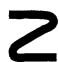
\includegraphics[keepaspectratio]{images/part001_0fdec0aa.jpg}}

测度 \(\lambda, \mu, \nu\) 定义在 \(G\) 上可能存在，使卷积积 \(\lambda * \mu\)、\((\lambda * \mu) * \nu\)、\(\mu * \nu\)、\(\lambda * (\mu * \nu)\) 都有定义，但仍有 \((\lambda * \mu) * \nu \neq \lambda * (\mu * \nu)\)（参见习题 4）。

设 \(\rho\) 是取有限值且 \(>0\) 的下半连续函数，定义在 \(\mathbf{G}\) 上，满足 \(\rho(st) \leqslant \rho(s)\rho(t)\) 对所有 \(s, t\) 在 \(\mathbf{G}\) 中成立。记 \(\mathcal{M}^{\rho}(\mathbf{G})\) 为由测度 \(\lambda\) 构成的向量空间，其中这些测度定义在 \(\mathbf{G}\) 上，且 \(\rho\) 对 \(\lambda\) 可积，并记 \(\|\lambda\|_{\rho}\)（或简写为 \(\|\lambda\|\)）为该空间上的范数 \(\int_{\mathbf{G}} \rho(s)d|\lambda|(s)\)。当 \(\rho = 1\) 时，就得到 \(\mathcal{M}^{1}(\mathbf{G})\)，即 \(\mathbf{G}\) 上有界测度的集合。

命题 2. --- (i) \(\mathcal{M}^{\rho}(\mathrm{G})\) 中任意两个元素都可卷积。

\begin{enumerate}
\def\labelenumi{(\roman{enumi})}
\setcounter{enumi}{1}
\item
  对于卷积和范数 \(\| \lambda \|\)，\(\mathcal{M}^{\rho}(\mathbf{G})\) 是完备赋范代数，并以 \(\varepsilon_{e}\) 为单位元。
\item
  \(\mathcal{C}'(\mathbf{G})\) 是 \(\mathcal{M}^{\rho}(\mathbf{G})\) 的子代数。
\end{enumerate}

设 \(\lambda, \mu\) 属于 \(\mathcal{M}^{\rho}(\mathbf{G})\)，我们来证明 \(\lambda\) 与 \(\mu\) 可卷积。设 \(f \in \mathcal{K}_{+}(\mathbf{G})\)。由于 \(\rho\) 是 \(>0\) 且下半连续的，存在常数 \(k > 0\) 使得 \(f \leqslant k\rho\)。于是

\[
\begin{array}{r l} & {\int^ {*} f (s t) d | \lambda | (s) d | \mu | (t) \leqslant k \int^ {*} \rho (s t) d | \lambda | (s) d | \mu | (t)} \\ & {\qquad \leqslant k \int^ {*} \rho (s) \rho (t) d | \lambda | (s) d | \mu | (t)} \\ & {\qquad = k \bigg (\int^ {*} \rho (s) d | \lambda | (s) \bigg) \bigg (\int^ {*} \rho (t) d | \mu | (t) \bigg)} \end{array}
\]

（第 V 章 §8 No.~3 命题 8 的推论 1）。因此，\((s,t) \mapsto f(st)\) 是 \((\lambda \otimes \mu)\)-可积的，从而 \(\lambda\) 与 \(\mu\) 可卷积。另一方面，利用第 V 章（§1 命题 4、§6 命题 2、§8 命题 8 的推论 1）以及 \((s,t) \mapsto \rho(s)\rho(t)\) 在 \(G \times G\) 上下半连续这一事实，有

\[
\begin{array}{r l} & {\int_ {\mathrm{G}} ^ {*} \rho (s) d | \lambda * \mu | (s) = \int_ {\mathrm{G}} ^ {\bullet} \rho (s) d | \lambda * \mu | (s)} \\ & {\quad \leqslant \int_ {\mathrm{G} \times \mathrm{G}} ^ {\bullet} \rho (s t) d | \lambda | (s) d | \mu | (t) \leqslant \int_ {\mathrm{G} \times \mathrm{G}} ^ {\bullet} \rho (s) \rho (t) d | \lambda | (s) d | \mu | (t)} \\ & {\quad = \int_ {\mathrm{G} \times \mathrm{G}} ^ {*} \rho (s) \rho (t) d | \lambda | (s) d | \mu | (t) = \| \lambda \| \cdot \| \mu \|.} \end{array}
\]

可见 \(\lambda * \mu \in \mathcal{M}^{\rho}(\mathrm{G})\)，且 \(\| \lambda * \mu \| \leqslant \| \lambda \| \cdot \| \mu \|\)。根据命题 1，\(\mathcal{M}^{\rho}(\mathrm{G})\) 是一个代数。映射 \(\lambda \mapsto \rho \cdot \lambda\) 是等距线性映射 \(\theta\)，将 \(\mathcal{M}^{\rho}(\mathrm{G})\) 映入 \(\mathcal{M}^{1}(\mathrm{G})\)；若 \(\mu \in \mathcal{M}^{1}(\mathrm{G})\)，则 \(1 / \rho\) 局部有界且上半连续，局部 \(\mu\)-可积，而 \(\rho\) 对 \((1 / \rho) \cdot \mu\) 可积，故 \((1 / \rho) \cdot \mu \in \mathcal{M}^{\rho}(\mathrm{G})\)；这证明了 \(\theta\) 是满射；因此 \(\mathcal{M}^{\rho}(\mathrm{G})\) 是完备赋范代数。最后，显然 \(\varepsilon_{e}\) 是 \(\mathcal{M}^{\rho}(\mathrm{G})\) 的单位元，且 \(\mathcal{C}'(\mathrm{G})\) 是 \(\mathcal{M}^{\rho}(\mathrm{G})\) 的子代数（§1 No.~4 命题 5 的推论）。

若 \(\rho = 1\)，命题 2 的 (i) 和 (ii) 也由 §1 的命题 2 得出。

命题 3. --- 设 \(\mu_1, \ldots, \mu_n\) 是 G 上的测度。若这些 \(\mu_i\) 中至多一个没有紧支集，则 \(\mu_i\) 可卷积。

事实上，令 \(S_{i}\) 为 \(\mu_{i}\) 的支集，并设 \(S_{i}\) 对 \(i \neq i_{0}\) 是紧的。令 K 为 G 的一个紧子集。满足 \((x_{1}, \ldots, x_{n}) \in \prod_{i} S_{i}\) 且 \(x_{1}x_{2} \cdots x_{n} \in K\) 的集合是紧的，因为条件 \(x_{i} \in S_{i}\) 对所有的 \(i, x_{1}x_{2} \cdots x_{n} \in K\) 均成立，蕴含

\[
x _ {i _ {0}} \in \mathrm{S} _ {i _ {0} - 1} ^ {- 1} \dots \mathrm{S} _ {1} ^ {- 1} \mathrm{KS} _ {n} ^ {- 1} \dots \mathrm{S} _ {i _ {0} + 1} ^ {- 1}.
\]

因此 \(\mu_{i}\) 可卷积（§1 No.~4 命题 4）。

命题 4. --- 映射 \((\lambda, \mu) \mapsto \lambda * \mu\)（分别为 \((\lambda, \mu) \mapsto \mu * \lambda)\)），其中 \(\lambda \in \mathcal{C}'(G)\)、\(\mu \in \mathcal{M}(G)\)，在 \(\mathcal{M}(G)\) 上定义了关于代数 \(\mathcal{C}'(G)\) 的左（分别为右）模结构。

这由命题 1 和命题 3 得出。

命题 5. --- 设 \(\lambda\) 是 G 上的左（分别为右）Haar 测度，且 \(\mu \in \mathcal{M}^1(\mathrm{G})\)。则 \(\mu\) 与 \(\lambda\)（分别为 \(\lambda\) 与 \(\mu\)）可卷积，且 \(\mu * \lambda = \mu(1)\lambda\)（分别为 \(\lambda * \mu = \mu(1)\lambda\)）。

不妨设 \(\mu \geqslant 0\)。令 \(f \in \mathcal{K}_{+}(\mathbf{G})\)。当 \(\lambda\) 是左 Haar 测度时，

\[
\int^ {*} d \mu (x) \int^ {*} f (x y) d \lambda (y) = \int^ {*} d \mu (x) \int f (y) d \lambda (y) = \lambda (f) \| \mu \|,
\]

因此函数 \((x,y)\mapsto f(xy)\) 是 \((\mu \otimes \lambda)\)-可积的，并且它关于 \(\mu \otimes \lambda\) 的积分为 \(\lambda (f)\| \mu \|\)。当 \(\lambda\) 是右 Haar 测度时，论证类似。

命题 6. --- 设 \(\mu\) 与 \(\nu\) 是 \(\mathbf{G}\) 上的两个可卷积测度。设 \(\chi\) 是 \(\mathbf{G}\) 在 \(\mathbf{C}^*\) 中的连续表示。则 \(\chi \cdot \mu\) 与 \(\chi \cdot \nu\) 可卷积，且 \((\chi \cdot \mu) * (\chi \cdot \nu) = \chi \cdot (\mu * \nu)\)。

令 \(f \in \mathcal{K}(\mathbf{G})\)。则 \(f\chi \in \mathcal{K}(\mathbf{G})\)，从而函数

\[
(x, y) \mapsto f (x y) \chi (x y) = f (x y) \chi (x) \chi (y)
\]

在 \(\mathbf{G} \times \mathbf{G}\) 上关于 \(\mu \otimes \nu\) 可积；因此函数 \((x, y) \mapsto f(xy)\) 关于 \((\chi \cdot \mu) \otimes (\chi \cdot \nu)\) 可积；所以 \(\chi \cdot \mu\) 与 \(\chi \cdot \nu\) 可卷积。此外，

\[
\begin{array}{r l} \langle \chi \cdot \mu * \chi \cdot \nu , f \rangle & = \int f (x y) \chi (x) \chi (y) d \mu (x) d \nu (y) \\ & = \int (f \chi) (x y) d \mu (x) d \nu (y) = \langle \mu * \nu , \chi f \rangle , \end{array}
\]

由此得到 \((\chi \cdot \mu) * (\chi \cdot \nu) = \chi \cdot (\mu * \nu)\)。

命题 7. --- 设 G 和 G' 是两个局部紧群，u 是 G 在 G' 中的连续表示，\(\mu_{1},\ldots,\mu_{n}\) 是 G 上均 \(\neq0\) 的测度。则下列断言等价：

\begin{enumerate}
\def\labelenumi{(\roman{enumi})}
\item
  \(u\) 对 \(\mu_{i}\) 是适当的，对所有 \(i\) 均如此，且测度 \(u(|\mu_i|)\) 可卷积；
\item
  \(\mu_{i}\) 可卷积，且 \(u\) 对 \(*_{i}(|\mu_{i}|)\) 是适当的
\end{enumerate}

满足这些条件时，

\[
\underset {i} {\ast} u (\mu_ {i}) = u \Big (\underset {i} {\ast} \mu_ {i} \Big).
\]

这由 §1 No.~2 命题 1 的推论得出。

推论。 --- 设 G 是局部紧群，\(\mu_{1},\ldots,\mu_{n}\) 是 G 上的测度。序列 \((\mu_{i})_{1\leqslant i\leqslant n}\) 可卷积的充要条件是序列 \((\breve{\mu}_{n-i})_{0\leqslant i\leqslant n-1}\) 可卷积；在此情形下，

\[
\left(\mu_ {1} * \dots * \mu_ {n}\right) ^ {\vee} = \stackrel {\vee} {\mu} _ {n} * \dots * \stackrel {\vee} {\mu} _ {1}.
\]

这是将同构 \(x \mapsto x^{-1}\) 从 \(G\) 到对立群应用于命题 7 的结果。

\subsection{群作用于空间的情形}

设 X 是局部紧空间，局部紧群 G 在其上连续地左作用，作用由

\[
(s, x) \mapsto s \cdot x.
\]

若 \(\mu_{1},\ldots,\mu_{n}\) 是 G 上的测度，\(\nu\) 是 X 上的测度，则称这些测度可卷积，是指它们对于映射 \((s_{1},\ldots,s_{n},x)\mapsto s_{1}\cdots s_{n}x\)，即从 \(G^{n}\times X\) 到 X 的映射，可卷积；它们的卷积积应按此映射的意义理解。

若 \(s\in \mathbf{G}\) 且 \(x\in \mathbf{X}\)，则

\[
\varepsilon_ {s} * \varepsilon_ {x} = \varepsilon_ {s x}.\tag{4}
\]

若 \(s \in \mathbf{G}\) 且 \(\mu \in \mathcal{M}(\mathbf{X})\)，则

\[
\varepsilon_ {s} * \mu = \gamma (s) \mu\tag{5}
\]

根据 §1 No.~1 的例 3。

命题 8. --- 设 \(\mu\) 是 G 上的测度，\(\nu\) 是 X 上的测度。

\begin{enumerate}
\def\labelenumi{(\roman{enumi})}
\item
  若 \(\mu\) 具有紧支集，则 \(\mu\) 与 \(\nu\) 可卷积。
\item
  若 \(\nu\) 具有紧支集，且 \(G\) 在 \(X\) 上适当作用，则 \(\mu\) 与 \(\nu\) 可卷积。
\end{enumerate}

这由 §1 No.~4 的命题 4 得出。

命题 9. --- 关于卷积，\(\mathcal{M}^{1}(\mathrm{X})\) 是 \(\mathcal{M}^{1}(\mathrm{G})\) 上的左模，而 \(\mathcal{M}(\mathrm{X})\) 和 \(\mathcal{C}'(\mathrm{X})\) 是 \(\mathcal{C}'(\mathrm{G})\) 上的左模。

这由命题 8 以及 §1 的命题 1、3 和命题 5 的推论得出。

命题 10. --- 设 \(\mu\) 是 \(G\) 上的测度，\(\nu\) 是 \(X\) 上的测度，且 \(\mu\) 与 \(\nu\) 可卷积。再假定存在正测度 \(\beta\)，定义在 \(X\) 上，使得 \(\gamma(s)\nu\) 以 \(\beta\) 为基，对每个 \(s \in G\) 都成立。则 \(\mu * \nu\) 以 \(\beta\) 为基。

令 K 是 X 的一个 \(\beta\)-零测紧子集。则 K 都是 \(\pmb{\gamma}(s)|\nu|\)-零测的，对每个 \(s \in G\) 均如此。现在，

\[
| \mu | * | \nu | = \int_ {\mathrm{G}} (\varepsilon_ {s} * | \nu |) d | \mu | (s)
\]

（§1 No.~5 命题 7），且映射 \(s \mapsto \varepsilon_s * |\nu|\) 弱连续（§2 命题 6）。因此根据第 V 章 §3 No.~3 定理 1，K 是 \(|\mu| * |\nu|\)-零测的。因此 \(|\mu| * |\nu|\) 以 \(\beta\) 为基（第 V 章 §5 No.~5 定理 2）。
